\documentclass[8pt]{beamer}
\usetheme{metropolis} % Use the Metropolis theme
\usepackage{pgfplots}
\usepackage{caption,subcaption}
\usepackage[style=authoryear,backend=biber]{biblatex}
\usepackage[table]{xcolor}
\addbibresource{../references.bib}

\title{Finite element analysis of multi-dimensional and simplified models for beams}
\author{Rudi du Toit}
\date{\today}
\institute{University of Pretoria}

\newcommand{\footfullcitenonumber}[1]{
  \footnotetext{\fullcite{#1}}
}

\begin{document}

% Redefine the title page template
\setbeamertemplate{title page}{
    \begin{center}
        \usebeamercolor[fg]{titlegraphic}\inserttitlegraphic\par
        \vskip0.25em%
        {\fontsize{14}{16}\selectfont\usebeamerfont{title}\usebeamercolor[fg]{title}\inserttitle\par}% Increase the font size of the title
        \ifx\insertsubtitle\@empty%
        \else%
        \vskip0.25em%
        {\fontsize{12}{14}\selectfont\usebeamerfont{subtitle}\usebeamercolor[fg]{subtitle}\insertsubtitle\par}% Increase the font size of the subtitle
        \fi%     
        \vskip1em\par
        \usebeamerfont{author}\insertauthor\par
        \vskip1em\par
        \usebeamerfont{institute}\insertinstitute\par
        \vskip1em%
        
\includegraphics[width=0.2\linewidth]{logo-up.jpg}\par % Include the logo here
        \vskip1em\par
        \usebeamerfont{date}\insertdate\par
        \vfill
    \end{center}
}



\begin{frame}[plain]
\titlepage
\end{frame}

\section{Introduction}
    \begin{frame}{Introduction}
        Beams are fundamental structural elements in engineering. They are used in a wide range of applications, from bridges to buildings.

        Simplified models are often used in vibration problems due to their reduced complexity and computational demand. However, the accuracy of these models in practical applications is not always certain.

        In this presentation, we look at the validity of the Timoshenko beam model as well as the validity of the two-dimensional model. We use modal analysis and the Finite Element Method (FEM) to compare the models' natural frequencies and mode shapes to those of a more realistic three-dimensional model.
    \end{frame}

    \begin{frame}{Structure of the presentation}
        \tableofcontents
    \end{frame}

\section{Literature study}
    \subsection{Comparison of linear beam theories}
        \begin{frame}{Literature study - Comparison of linear beam theories}
            Consider the article \textit{Comparison of linear beam theories} [\cite{LVV09}]
            
            \textbf{Objective of Comparison:}
            \begin{itemize}
              \item To validate the efficacy of the Timoshenko beam theory against a more realistic two-dimensional model.
            \end{itemize}
            
            \textbf{Methodology:}
            \begin{itemize}
              \item Use modal analysis and the Finite Element Method (FEM) to calculate natural frequencies and modes, providing a direct comparison of results from both models.
            \end{itemize}
            
            \textbf{Key Findings:}
            \begin{itemize}
              \item Timoshenko model results closely match those from the two-dimensional model, especially for the first ten eigenvalues.
              \item The shape of the beams significantly influences the accuracy of the Timoshenko model.
            \end{itemize}

            \footfullcite{LVV09}
        \end{frame}
            
        \begin{frame}{Literature study - Comparison of linear beam theories}
            
            \textbf{Conclusions and Recommendations:}
            \begin{itemize}
              \item For practical applications, the Timoshenko beam model is a suitable approximation for two-dimensional model.
              \item This article excluded damping.
              \item This comparison serves as an intermediate step towards the more comprehensive analysis involving the comparison of Timoshenko beam model and a three-dimensional model. A direct comparison is preferred but this will introduce additional complexities.
            \end{itemize}

            \textbf{In this presentation:}
            \begin{itemize}
              \item We will replicate the results of this article using the Finite Element Method (FEM) and modal analysis.
              \item We will improve the results by increasing the accuracy to 5 significant digits.
              \item We extent the article to also include the comparison of the two-dimensional model with a three-dimensional model.
            \end{itemize}
            
        \end{frame}


    \subsection{Empirical comparison of beams}
        \begin{frame}{Literature study - Empirical comparison of beams}
            Consider the article \textit{On the valid frequency range of Timoshenko beam theory} [\cite{SP06}]

            \textbf{Objective:}
            \begin{itemize}
                \item To validate the frequency predictions of Timoshenko beam theory for different end conditions and frequencies.
            \end{itemize}
        
            \textbf{Methodology:}
            \begin{itemize}
                \item Experimental setup involved a short free-free beam of near-square cross-section.
                \item Beam dimensions: Length = 40.047 mm, Breadth = 10.097 mm, Depth = 10.047 mm.
                \item Beam material: Aluminum alloy, with properties determined via resonant ultrasound spectroscopy (RUS).
                \item Comparisons made with experimental observations, commercial finite element (ANSYS) predictions, and RUS technique predictions.
                \item Finite element analysis used 20-node brick elements, and TBT predictions were calculated using specific frequency equations.
            \end{itemize}

            \footfullcite{SP06}
        \end{frame}

        \begin{frame}{Setup and Testing Method}
            
        
            \textbf{Key Setup Features:}
            \begin{itemize}
                \item The experimental beam was suspended and excited by two carbon-fibre loops attached to piezoelectric transducers.
                \item Resonant frequencies detected by sweeping the frequency range with a network analyzer.
            \end{itemize}

            \begin{figure}[h!]
                \centering
                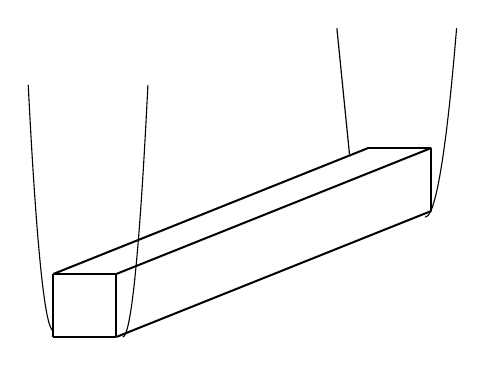
\begin{tikzpicture}[scale=0.8]
                    
                    \draw[line width = 0.25mm] (2,0) -- (7,2);
                    \draw[line width = 0.25mm] (2,1) -- (7,3);
                    \draw[line width = 0.25mm] (1,1) -- (6,3);
                    
                    \draw[line width = 0.25mm] (2,0) -- (2,1);
                    \draw[line width = 0.25mm] (1,0) -- (1,1);
                    \draw[line width = 0.25mm] (2,0) -- (1,0);
                    \draw[line width = 0.25mm] (2,1) -- (1,1);
                    
                    \draw[line width = 0.25mm] (6,3) -- (7,3);
                    \draw[line width = 0.25mm] (7,3) -- (7,2);
                    
                    \draw(2.1,0) parabola (2.5,4);
                    \draw(1,0.1) parabola (0.6,4);
                    
                    \draw(6.9,1.9) parabola (7.4,4.9);
                    \draw[line width = 0.15mm] (5.7,2.9) -- (5.5,4.9);
                
                \end{tikzpicture}
            \end{figure} 
        \end{frame}
        
        \begin{frame}{Numerical Results and Discussion}
            \textbf{Results Summary:}
            \begin{itemize}
                \item Excellent agreement between measured, ANSYS, and RUS frequencies below the cut-off frequency.
            \end{itemize}

            \textbf{Some results from the article:}
            \begin{table}[htbp]
                \makebox[\textwidth]{
                \begin{tabular}{||c|c|cc|cc|c||}
                    \hline
                    {n} & {Measured} & {3D FEM} & {\% Error} & {Timoshenko Beam} & {\% Error} & Side \\
                    \hline
                    1     & 27359.6 & 27417.6 & 0,21\% & 27407.1 & 0,17\% & Flexible \\
                            & 27423.8 & 27515.6 & 0,33\% & 27505.3 & 0,30\% & Stiff \\
                    2     & 60862   & 60882.0 & 0,03\% & 60851.1 & -0,02\% & Flexible \\
                           & 61098.3 & 61022.0 & -0,12\% & 60992.1 & -0,17\% & Stiff \\
                    3     & 97609.5 & 97734.4 & 0,13\% & 97796.0 & 0,19\% & Flexible \\
                          & 97852.4 & 97881.5 & 0,03\% & 97945.4 & 0,09\% & Stiff \\
                    4     & 161494 & 131658 & 0,12\% & 132277 & 0,60\% & Flexible \\
                          & 131732 & 131675 & -0,04\% & 132308 & 0,44\% & Stiff \\
                    5     & 161352 & 161390 & 0,02\% & 163547 & 1,36\% & Stiff \\
                          & 161538 & 161517 & -0,01\% & 163611 & 1,31\% & Flexible \\
                    6     & 165183 & 164887 & -0,18\% & 169108 & 2,38\% & Stiff \\
                          & 165598 & 165398 & -0,12\% & 169634 & 2,44\% & Flexible \\
                    7     & 194863 & 194933 & 0,04\% & 202352 & 3,84\% & Flexible \\
                             & 194973 & 195032 & 0,03\% & 202115 & 3,66\% & Stiff \\
                    8     & 195869 & 195977 & 0,06\% & 203319 & 3,80\% & Stiff \\
                          & 195908 & 196097 & 0,10\% & 203518 & 3,88\% & Flexible \\
                    9     & 213501 &       &       & 241202 & 12,97\% & Flexible \\
                          & 213635 &       &       & 241067 & 12,84\% & Stiff \\
              {10 and 11} & 220556 &       &       & 247954 & 12,42\% & Flexible \\
                          & 220702 &       &       & 281542 & 27,57\% & Flexible \\
                          & 221010 &       &       & 247782 & 12,11\% & Stiff \\
                          & 221092 &       &       & 281408 & 27,28\% & Stiff \\
                    \hline
                \end{tabular}%
            }
            \end{table}%
        \end{frame}
        


\section{Models}
    \subsection{Timoshenko cantilever beam}
        \begin{frame}{Models - Timoshenko cantilever beam}
            \begin{columns}[T] % align columns
                \begin{column}{.6\textwidth}
                    \only<1->{ % Frame 1: Equations of motion
                    Equations of motion
                    \begin{eqnarray*}
                        \partial_{t}^{2} w &=& \partial_{x}V + Q,\\
                        \frac{1}{\alpha} \partial_{t}^{2} \phi &=& V + \partial_{x}M.
                    \end{eqnarray*}
                    % Frame 1: Constitutive equations
                    Constitutive equations
                    \begin{eqnarray*}
                        M &=& \frac{1}{\beta}\partial_x \phi,\\
                        V &=& \partial_x w-\phi.
                    \end{eqnarray*}
                    }
                \end{column}
                
                \begin{column}{.4\textwidth}
                    \only<2->{% Frame 2: Parameter descriptions
                    \textbf{Description:}
                    \begin{itemize}
                        \item[-] \( w \): Displacement
                        \item[-] \( \phi \): Angle of rotation of the cross-sections
                        \item[-] \( M \): Bending moment
                        \item[-] \( V \): Shear force
                        \item[-] \( Q \): External distributed load
                        \item[-] \( \alpha, \beta \): Dimensionless constants
                    \end{itemize}}
                \end{column}
            \end{columns}
        \end{frame}

        \begin{frame}{Models - Timoshenko cantilever beam}
            \begin{figure}[h!]
                \centering
                \begin{tikzpicture}
                    
                    \draw[line width = 0.4mm] (0,0) -- (6,0);
                    \node at (2.7,-0.25) {$\ell = 1$};
                    
                    \draw[line width = 0.1mm] (0,-1.5) -- (0,1.5);
                    \draw[line width = 0.1mm] (0,1.5) -- (-0.2,1.4);
                    \draw[line width = 0.1mm] (0,1.3) -- (-0.2,1.2);
                    \draw[line width = 0.1mm] (0,1.1) -- (-0.2,1);
                    \draw[line width = 0.1mm] (0,0.9) -- (-0.2,0.8);
                    \draw[line width = 0.1mm] (0,0.7) -- (-0.2,0.6);
                    \draw[line width = 0.1mm] (0,0.5) -- (-0.2,0.4);
                    \draw[line width = 0.1mm] (0,0.3) -- (-0.2,0.2);
                    \draw[line width = 0.1mm] (0,0.1) -- (-0.2,0);
                    \draw[line width = 0.1mm] (0,-0.1) -- (-0.2,-0.2);
                    \draw[line width = 0.1mm] (0,-0.3) -- (-0.2,-0.4);
                    \draw[line width = 0.1mm] (0,-0.5) -- (-0.2,-0.6);
                    \draw[line width = 0.1mm] (0,-0.7) -- (-0.2,-0.8);
                    \draw[line width = 0.1mm] (0,-0.9) -- (-0.2,-1);
                    \draw[line width = 0.1mm] (0,-1.1) -- (-0.2,-1.2);
                    \draw[line width = 0.1mm] (0,-1.3) -- (-0.2,-1.4);
                    \draw[line width = 0.1mm] (0,-1.5) -- (-0.2,-1.6);
                    
                    % Adding points 0 and 1
                    \node at (0,-0.35) {0};
                    \node at (6,-0.35) {1};
                    
                \end{tikzpicture}
                \caption{A cantilever Timoshenko beam.}
            \end{figure} 
        
            Boundary conditions for a cantilever beam
            \begin{eqnarray*}
                w(0,\cdot) = 0, &\phi(0,\cdot) = 0,\\
                M(1,\cdot) = 0, &V(1,\cdot) = 0.
            \end{eqnarray*}
        \end{frame}

    \subsection{Two-dimensional cantilever beam}
        \begin{frame}{Models - Two-dimensional cantilever beam}
            \begin{columns}[T] % align columns
                \begin{column}{.6\textwidth}
                    \only<1->{ % Frame 1: Equations of motion
                        Equations of motion
                        \begin{eqnarray*}
                            \partial_t^2 u & = & \textrm{div}T + Q,
                        \end{eqnarray*}
                        with
                        \begin{eqnarray*}
                            \textrm{div} T & = &
                            \begin{bmatrix}
                                \partial_1 \sigma_{11} + \partial_2 \sigma_{12} \\
                                \partial_1 \sigma_{21} + \partial_2 \sigma_{22}
                            \end{bmatrix}.
                        \end{eqnarray*}
                    }
                    \only<1->{ % Frame 1: Constitutive equations
                        Constitutive equations
                        \begin{eqnarray*}
                            T = \frac{1}{\gamma(1+\nu)}\mathcal{E} + \frac{\nu}{\gamma(1-\nu^2)}\textrm{tr}(\mathcal{E}) I
                        \end{eqnarray*}
                    }
                \end{column}
                
                \begin{column}{.4\textwidth}
                    \only<2->{ % Frame 2: Parameter descriptions
                        \textbf{Description:}
                        \begin{itemize}
                            \item[-] \( u \): Displacement vector in 2D
                            \item[-] \( T \): Stress tensor
                            \item[-] \( Q \): External distributed load in 2D
                            \item[-] \( \mathcal{E} \): Young's modulus
                            \item[-] \( \nu \): Poisson's ratio
                            \item[-] \( \gamma \): Dimensionless constant
                        \end{itemize}
                    }
                \end{column}
            \end{columns}
        \end{frame}

        \begin{frame}{Models - Two-dimensional cantilever beam}
            \begin{figure}[h!]
                \centering
                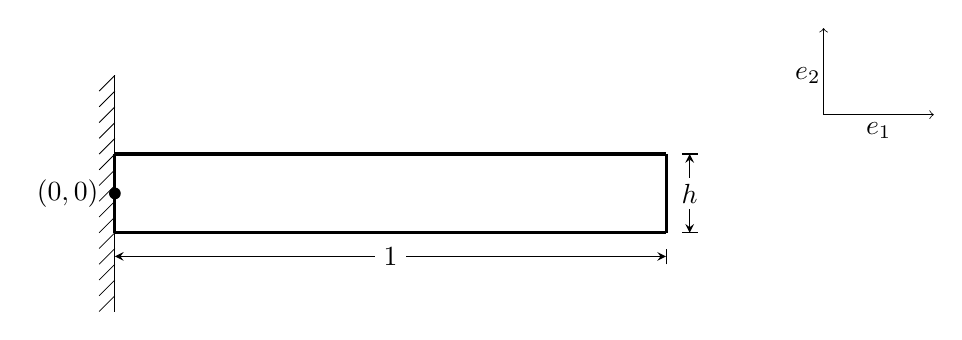
\begin{tikzpicture}
                    
                    \draw[line width = 0.4mm] (0,0.5) -- (7,0.5);
                    \draw[line width = 0.4mm] (0,-0.5) -- (7,-0.5);
                    \draw[line width = 0.4mm] (7,-0.5) -- (7,0.5);
                    \draw[line width = 0.4mm] (0,-0.5) -- (0,0.5);
                    
                    \draw[line width = 0.1mm] (0,1.5) -- (0,-1.5);
                    
                    \draw[line width = 0.1mm] (0,1.5) -- (-0.2,1.3);
                    \draw[line width = 0.1mm] (0,1.3) -- (-0.2,1.1);
                    \draw[line width = 0.1mm] (0,1.1) -- (-0.2,0.9);
                    \draw[line width = 0.1mm] (0,0.9) -- (-0.2,0.7);
                    \draw[line width = 0.1mm] (0,0.7) -- (-0.2,0.5);
                    \draw[line width = 0.1mm] (0,0.5) -- (-0.2,0.3);
                    \draw[line width = 0.1mm] (0,0.3) -- (-0.2,0.1);
                    \draw[line width = 0.1mm] (0,0.1) -- (-0.2,-0.1);
                    \draw[line width = 0.1mm] (0,-0.1) -- (-0.2,-0.3);
                    \draw[line width = 0.1mm] (0,-0.3) -- (-0.2,-0.5);
                    \draw[line width = 0.1mm] (0,-0.5) -- (-0.2,-0.7);
                    \draw[line width = 0.1mm] (0,-0.7) -- (-0.2,-0.9);
                    \draw[line width = 0.1mm] (0,-0.9) -- (-0.2,-1.1);
                    \draw[line width = 0.1mm] (0,-1.1) -- (-0.2,-1.3);
                    \draw[line width = 0.1mm] (0,-1.3) -- (-0.2,-1.5);
                    
                    \node at (7.3,0) {$h$};
                    \draw[-stealth] (7.3,0.2) -- (7.3,0.5);
                    \draw (7.2,0.5) -- (7.4,0.5);
                    \draw[-stealth] (7.3,-0.2) -- (7.3,-0.5);
                    \draw (7.2,-0.5) -- (7.4,-0.5);
                    
                    \node at (3.5,-0.8) {$1$};
                    \draw[stealth-] (0,-0.8) -- (3.3,-0.8);
                    \draw[stealth-] (7,-0.8) -- (3.7,-0.8);
                    \draw (7,-0.9) -- (7,-0.7);
                    
                    \draw[line width = 0.1mm,->] (9,1) -- (10.4,1);
                    \draw[line width = 0.1mm,->] (9,1) -- (9,2.1);
                    \node at (9.7,0.8) {$e_1$};
                    \node at (8.8,1.5) {$e_2$};
                    
                    \node at (-0.6,0) {$(0,0)$};
                    \node at (0,0)[circle,fill,inner sep=1.5pt]{};
                    
                \end{tikzpicture}
                \caption{A cantilever two-dimensional elastic body.}
            \end{figure} 
        
            % Placeholder for boundary conditions of 2D cantilever
            Boundary Conditions:
            \begin{eqnarray*}
                u & = & 0 \quad \textrm{ where } x_1 = 0\\
                Tn & = & 0 \quad \textrm{ on the rest of the body }
            \end{eqnarray*} With $n$ the outward normal vector to $\Omega$.
        \end{frame}

    \subsection{Three-dimensional cantilever beam}
        \begin{frame}{Models - Three-dimensional cantilever beam}
            \begin{columns}[T] % align columns
                \begin{column}{.6\textwidth}
                    \only<1->{ % Frame 1: Equations of motion
                        Equations of motion
                        \begin{eqnarray*}
                            \partial_t^2 u & = & \textrm{div}T + Q
                        \end{eqnarray*}
                        with
                        \begin{eqnarray*}
                            \textrm{div}  T & = &
                            \begin{bmatrix}
                                \partial_1 \sigma_{11} + \partial_2 \sigma_{12} + \partial_3 \sigma_{13} \\
                                \partial_1 \sigma_{21} + \partial_2 \sigma_{22} + \partial_3 \sigma_{23} \\
                                \partial_1 \sigma_{31} + \partial_2 \sigma_{32} + \partial_3 \sigma_{33}
                            \end{bmatrix}.\label{eq:3D_Model:divT-D}
                        \end{eqnarray*}
                    }
                    \only<1->{ % Frame 1: Constitutive equations
                        Constitutive equations
                        \begin{eqnarray*}
                            T = \frac{1}{\gamma(1+\nu)} \mathcal{E} + \frac{\nu}{\gamma(1+\nu)(1-2\nu)}\textrm{Tr}(\mathcal{E})I
                        \end{eqnarray*}
                    }
                \end{column}
                
                \begin{column}{.4\textwidth}
                    \only<2->{ % Frame 2: Parameter descriptions
                        \textbf{Description:}
                        \begin{itemize}
                            \item[-] \( u \): Displacement vector in 2D
                            \item[-] \( T \): Stress tensor
                            \item[-] \( Q \): External distributed load in 2D
                            \item[-] \( \mathcal{E} \): Young's modulus
                            \item[-] \( \nu \): Poisson's ratio
                            \item[-] \( \gamma \): Dimensionless constant
                        \end{itemize}
                    }
                \end{column}
            \end{columns}
        \end{frame}

        \begin{frame}{Models - Three-dimensional cantilever beam}
            Assume that $\sigma_{3i} = 0$ for $i = 1, 2, 3$; $\partial_3 u_1 = 0$, $\partial_3 u_2 = 0$ ($u_1$ and $u_2$ are functions of $x_1$ and $x_2$), and the strain component $\varepsilon_{33} = 0$. Then using the definition of strain 
            \begin{eqnarray}
                \partial_i u_3 = 0 \quad \textrm{ for } i = 1,2,3 \textrm{ on } \Omega.
            \end{eqnarray}

            It follows that $u_3$ is a constant on $\Omega$ and $u$ is a vector valued function in $R^2$ with two-dimensional stress and strain. The out of plane conditions for strain \eqref{plane_stress_neseccary_condition} falls away and Hooke’s law can be written in a two-dimensional form using the stress components (1.2.16) as $\displaystyle T = \frac{1}{\gamma(1+\nu)}\mathcal{E} + \frac{\nu}{\gamma(1-\nu^2)}\textrm{tr}(\mathcal{E})I.$\\


            
        \end{frame}

        \begin{frame}{Models - Three-dimensional cantilever beam}
            \begin{figure}[h!]
                \centering
                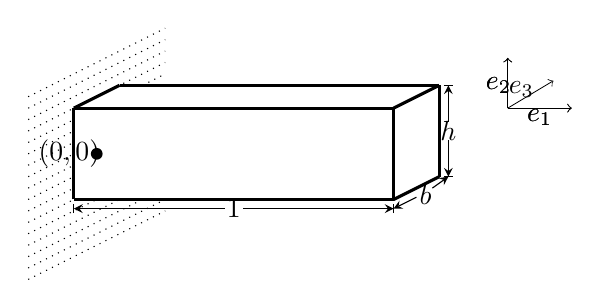
\begin{tikzpicture}[scale=0.58]
                    
                    \draw[line width = 0.4mm] (-0.5,1) -- (6.5,1);
                    \draw[line width = 0.4mm] (-0.5,-1) -- (6.5,-1);
                    \draw[line width = 0.4mm] (6.5,-1) -- (6.5,1);
                    \draw[line width = 0.4mm] (-0.5,-1) -- (-0.5,1);
                    
                    \draw[line width = 0.4mm] (0.5,1.5) -- (7.5,1.5);
                    \draw[line width = 0.4mm] (7.5,-0.5) -- (7.5,1.5);
                    
                    
                    \draw[line width = 0.4mm] (-0.5,1) -- (0.5,1.5);
                    \draw[line width = 0.4mm] (6.5,1) -- (7.5,1.5);
                    \draw[line width = 0.4mm] (6.5,-1) -- (7.5,-0.5);
                    
                    
                    
                    \draw[scale=0.5, domain=-3:3, smooth, variable=\x,dotted] plot ({\x}, {0.5*\x+4});
                    \draw[scale=0.5, domain=-3:3, smooth, variable=\x,dotted] plot ({\x}, {0.5*\x+3.5});
                    \draw[scale=0.5, domain=-3:3, smooth, variable=\x,dotted] plot ({\x}, {0.5*\x+3});
                    \draw[scale=0.5, domain=-3:3, smooth, variable=\x,dotted] plot ({\x}, {0.5*\x+2.5});
                    
                    \draw[scale=0.5, domain=-3:-1, smooth, variable=\x,dotted] plot ({\x}, {0.5*\x+2});
                    \draw[scale=0.5, domain=2:3, smooth, variable=\x,dotted] plot ({\x}, {0.5*\x+2});
                    
                    \draw[scale=0.5, domain=-3:-1, smooth, variable=\x,dotted] plot ({\x}, {0.5*\x+1.5});
                    \draw[scale=0.5, domain=-3:-1, smooth, variable=\x,dotted] plot ({\x}, {0.5*\x+1});
                    \draw[scale=0.5, domain=-3:-1, smooth, variable=\x,dotted] plot ({\x}, {0.5*\x+0.5});
                    \draw[scale=0.5, domain=-3:-1, smooth, variable=\x,dotted] plot ({\x}, {0.5*\x});
                    \draw[scale=0.5, domain=-3:-1, smooth, variable=\x,dotted] plot ({\x}, {0.5*\x-0.5});
                    \draw[scale=0.5, domain=-3:-1, smooth, variable=\x,dotted] plot ({\x}, {0.5*\x-1});
                    \draw[scale=0.5, domain=-3:-1, smooth, variable=\x,dotted] plot ({\x}, {0.5*\x-1.5});
                    \draw[scale=0.5, domain=-3:0, smooth, variable=\x,dotted] plot ({\x}, {0.5*\x-2});
                    \draw[scale=0.5, domain=-3:1, smooth, variable=\x,dotted] plot ({\x}, {0.5*\x-2.5});
                    \draw[scale=0.5, domain=-3:2, smooth, variable=\x,dotted] plot ({\x}, {0.5*\x-3});
                    \draw[scale=0.5, domain=-3:3, smooth, variable=\x,dotted] plot ({\x}, {0.5*\x-3.5});
                    \draw[scale=0.5, domain=-3:3, smooth, variable=\x,dotted] plot ({\x}, {0.5*\x-4});
                    
                    %\node at (6.9,1) {$b$};
                    %\node at (6.65,0) {$h$};
                    %\node at (3.2,-1.2) {$\ell = 1$};
                    
                    \draw[line width = 0.1mm,->] (9,1) -- (10,1.6);
                    \draw[line width = 0.1mm,->] (9,1) -- (10.4,1);
                    \draw[line width = 0.1mm,->] (9,1) -- (9,2.1);
                    \node at (9.3,1.4) {$e_3$};
                    \node at (9.7,0.8) {$e_1$};
                    \node at (8.8,1.5) {$e_2$};
                    
                    \node at (7.7,0.5) {$h$};
                    \draw[-stealth] (7.7,0.7) -- (7.7,1.5);
                    \draw (7.6,1.5) -- (7.8,1.5);
                    \draw[-stealth] (7.7,0.3) -- (7.7,-0.5);
                    \draw (7.6,-0.5) -- (7.8,-0.5);
                    
                    \node at (3,-1.2) {$1$};
                    \draw[stealth-] (-0.5,-1.2) -- (2.8,-1.2);
                    \draw[stealth-] (6.5,-1.2) -- (3.2,-1.2);
                    \draw (6.5,-1.3) -- (6.5,-1.1);
                    \draw (-0.5,-1.3) -- (-0.5,-1.1);
                    
                    \node at (7.2,-0.9) {$b$};
                    \draw[stealth-] (7.7,-0.5) -- (7.35,-0.75);
                    \draw[stealth-] (6.5,-1.2) -- (7,-0.95);
                    
                    \draw[line width = 0.1mm,->] (9,1) -- (10.4,1);
                    \draw[line width = 0.1mm,->] (9,1) -- (9,2.1);
                    \node at (9.7,0.8) {$e_1$};
                    \node at (8.8,1.5) {$e_2$};
                    
                    \node at (-0.6,0) {$(0,0)$};
                    \node at (0,0)[circle,fill,inner sep=1.5pt]{};
                    
                    %\node at (-1.4,-1.3) {$(0,-\frac{h}{2},-\frac{b}{2})$};
                    %\node at (-1.4,1) {$(0,\frac{h}{2},-\frac{b}{2})$};
                    %\node at (0.5,1.8) {$(0,\frac{h}{2},\frac{b}{2})$};
                    
                    %\node at (6,-1.3) {$(1,-\frac{h}{2},-\frac{b}{2})$};
                    %\node at (6.3,0.7) {$(1,\frac{h}{2},-\frac{b}{2})$};
                    %\node at (7.5,1.8) {$(1,\frac{h}{2},\frac{b}{2})$};
                    %\node at (8.4,-0.4) {$(1,-\frac{h}{2},\frac{b}{2})$};
                    
                \end{tikzpicture}
                \caption{Cantilever Three-Dimensional Elastic Body with Rectangular Cross-Section.}
            \end{figure} 
            Boundary Conditions:
            \begin{eqnarray*}
                u & = & 0 \quad \textrm{ where } x_1 = 0\\
                Tn & = & 0 \quad \textrm{ on the rest of the body }
            \end{eqnarray*} With $n$ the outward normal vector to $\Omega$.
        \end{frame}

\section{Theory}
    \subsection{General vibration problem}
        \begin{frame}{General vibration problem}
            Let $V$, $W$ and $X$ be real Hilbert spaces such that $W$ is a linear subspace of $X$, and $V$ is a linear subspace of $W$, i.e. $V \subset W \subset X$.
            \begin{itemize}
                \item[] X is the global space with inner product $(\cdot,\cdot)_X$ and the induced norm $||\cdot||_X$.
                \item[] W is the inertia space with inner product $(\cdot,\cdot)_W$ and the induced norm $||\cdot||_W$.
                \item[] V is the energy space with inner product $(\cdot,\cdot)_V$ and the induced norm $||\cdot||_V$.
            \end{itemize}
            \only<2->{
            The bilinear forms $a$, $b$ and $c$ are defined as $a = (\cdot,\cdot)_X$,$b = (\cdot,\cdot)_V$ and $c = (\cdot,\cdot)_W$.
            }

            \only<3>{
            \textbf{General vibration problem:}
        
            Find a function $u \in C(J,\ X)$ such that $u'$ is continuous at $0$ with respect to $\Vert \cdot \Vert_{W}$, and for each $t \in J$, $u(t) \in V$, $u'(t) \in V$, $u''(t) \in W$, satisfying
            \begin{eqnarray}
                c(u''(t),v)+a(u'(t),v)+b(u(t),v) = (f(t),v) \ \ \ \ \textrm{for each} \ v \in V, \label{eq:existence:ProblemGVarHom}
            \end{eqnarray}
            with initial conditions $u(0) = u_0$ and $u'(0) = u_1$.}

            \only<4->{
            \textbf{General vibration problem:}
        
            Find a function $u \in C(J,\ X)$ such that $u'$ is continuous at $0$ with respect to $\Vert \cdot \Vert_{W}$, and for each $t \in J$, $u(t) \in V$, $u'(t) \in V$, $u''(t) \in W$, satisfying
            \begin{eqnarray}
                c(u''(t),v)+b(u(t),v) = (f(t),v) \ \ \ \ \textrm{for each} \ v \in V, \label{eq:existence:ProblemGVarHom}
            \end{eqnarray}
            with initial conditions $u(0) = u_0$ and $u'(0) = u_1$.}

            \footfullcitenonumber{VV02}
        \end{frame}

    \subsection{Existence and uniqueness of solutions}
        \begin{frame}{Existence and uniqueness of solutions}
            In [\cite{VV02}] the authors present results for the existence and uniqueness of solutions to the general vibration problem. The following assumptions are made for the existence results.

            \begin{itemize}
                \item[] \textbf{A1} - $V$ is dense in $W$ and $W$ is dense in $X$.

                \item[] \textbf{A2} - There exists a positive constant $C_{W}$ such that $\Vert w\Vert_{X} \leq C_{W}\Vert w\Vert_{W}$ for each $ w\in W$.

                \item[] \textbf{A3} - There exists a positive constant $C_{V}$ such that $\Vert v\Vert_{W} \leq C_{V}\Vert v\Vert_{V}$ for each $v \in V$.

                \item[] \textbf{A4} - The bilinear form $a$ is non-negative, symmetric and bounded on $V$, i.e. there exists a positive constant $K_a$ such that for $\displaystyle u,v \in V$, \[|a(u,v)| \leq K_a\Vert u \Vert_V \Vert v \Vert_V.\]
            \end{itemize}
            \footfullcitenonumber{VV02}
        \end{frame}

        \begin{frame}{Existence and uniqueness of solutions}
            \newtheorem{Thmx}{Theorem}
            \begin{Thmx}
                Suppose assumptions \textbf{A1}-\textbf{A4} hold. If, for $u_0 \in V$ and $u_1 \in V$, there exists some $y \in W$ such that
                \begin{eqnarray}
                    b(u_0,v) + a(u_1,v) = c(y,v) \ \ \ \ \textrm{ for all } \ v \in V, \label{bilinear_equation}
                \end{eqnarray}
                then for each $f \in C^1(J,X)$, there exists a unique solution $u \in C^1(J,V)\cap C^2(J,W)$ for Problem GVar.
            \end{Thmx}

            This theorem allows for a solution of the abstract variational problem Problem GVar, if the assumptions \textbf{A1}-\textbf{A4} is satisfied and the initial values $u_0$ and $u_1$ are admissible. It is not always easy to verify that \eqref{bilinear_equation} is satisfied.

            \footfullcitenonumber{VV02}
        \end{frame}


    \subsection{Modal Analysis}
        \begin{frame}{Modal Analysis}
            \textbf{General vibration problem:}
        
            Find a function $u \in C(J,\ X)$ such that $u'$ is continuous at $0$ with respect to $\Vert \cdot \Vert_{W}$, and for each $t \in J$, $u(t) \in V$, $u'(t) \in V$, $u''(t) \in W$, satisfying
            \begin{eqnarray}
                c(u''(t),v)+b(u(t),v) = 0 \ \ \ \ \textrm{for each} \ v \in V, \label{eq:existence:ProblemGVarHom}
            \end{eqnarray}
            with initial conditions $u(0) = u_0$ and $u'(0) = u_1$.
        
            \only<2->{
            Trial solution:
        
            $u(t) = T(t)x$ with $x \in V$ and $x \neq 0$}
        \end{frame}
        
        \begin{frame}{Modal Analysis}
           Substituting trial solution into \eqref{eq:existence:ProblemGVarHom}:
           \begin{eqnarray*}
                b(T(t)x,v) = - c(T''(t)x,v).  \label{eq:existence:ProblemGVarHom:Substitution}
            \end{eqnarray*}
        
            Due to the linearity of the bilinear form, this equation can be rewritten as
            \begin{eqnarray*}
                T(t)b(x,v) = - T''(t)c(x,v).
            \end{eqnarray*}
        
            \only<1>{
            Dividing both sides by $T(t)$ gives
            \begin{eqnarray*}
                b(x,v) = - \frac{T''(t)}{T(t)}c(x,v).
            \end{eqnarray*}}
        
            \only<2->{
            Dividing both sides by $T(t)$ gives
            \begin{eqnarray*}
                b(x,v) = - \frac{T''(t)}{T(t)}c(x,v) \implies  \frac{T''(t)}{T(t)} \ \ \ \textrm{must be constant.}
            \end{eqnarray*}}

            \only<3->{
                Set $\displaystyle \frac{T''(t)}{T(t)} = -\lambda$.
        
            At this point we do not yet know if such a $\lambda$ exists.
            }
        \end{frame}
        
        \begin{frame}{Modal Analysis}
            Eigenvalue Problem:
        
            Find a real number $\lambda$ and a $x \in V$ with $x \neq 0$ such that
            \begin{eqnarray}
                b(x,y) = \lambda c(x,y) \ \ \ \ \textrm{ for each } \ y \in V.
            \end{eqnarray}

            Ordinary differential equation for $T(t)$:
            \begin{eqnarray}
                T''(t)  + \lambda T(t) = 0. \label{eq:1D_Model:ModalAnalysisODE}
            \end{eqnarray}
         \end{frame}
        
        \begin{frame}{Modal Analysis}
            Assumptions:
            \begin{itemize}
                \item[] \textbf{A1} - $V$ is dense in $W$ and $W$ is dense in $X$.
            
                \item[] \textbf{A2} - There exists a positive constant $C_{W}$ such that $\Vert w\Vert_{X} \leq C_{W}\Vert w\Vert_{W}$ for each $ w\in W$.
            
                \item[] \textbf{A3} - There exists a positive constant $C_{V}$ such that $\Vert v\Vert_{W} \leq C_{V}\Vert v\Vert_{V}$ for each $v \in V$.
            
                \item[] \textbf{A4} - The bilinear form $a$ is non-negative, symmetric and bounded on $V$, i.e. there exists a positive constant $K_a$ such that for $\displaystyle u,v \in V$, \[|a(u,v)| \leq K_a\Vert u \Vert_V \Vert v \Vert_V.\]
            
                \item[] \alert{\textbf{A5} - The embedding of $V$ into $W$ is compact.} [\cite{CVV18}]
            \end{itemize}
            \footfullcite{CVV18}
        \end{frame}

        \begin{frame}{Modal Analysis}
            
            Using these assumptions, the authors prove that there exists a complete orthonormal sequence of eigenvectors for the eigenvalue problem with a corresponding sequence of eigenvalues. These eigenvalues are positive and the orthogonality is with respect to the bilinear form $c$. Also the sequence of normalized eigenvectors ${x_i}$ forms an orthonormal basis in $W$ and sequence of eigenvalues ${\lambda_i}$ is an infinite sequence with $\lambda_n \rightarrow \infty$ as $n \rightarrow \infty$. 
            
            Following these results, for any $u \in V$, $\displaystyle u = \sum_{i=1}^{\infty} a_i x_i$. These coefficients $a_i$ are generalized Fourier coefficients of $u$ with respect to the eigenvectors $x_i$. Therefore, for any $u \in V$,
            \begin{eqnarray*}
                u = \sum_{i=1}^{\infty} a_i x_i = \sum_{i=1}^{\infty} c(u, x_i)x_i.
            \end{eqnarray*}
            
            Now that the eigenvalue problem has many solutions, the following ordinary differentiable equation can be considered,
            \begin{eqnarray*}
                T_n'' + \lambda T_n = 0. 
            \end{eqnarray*}
        \end{frame}

        \begin{frame}
            Since this differential equation is a simple second order differential equation, $T_n(t)$ has the following possible solutions:
            \begin{flalign}
                T_n(t) &=  A_n \cos(\sqrt{\lambda_n} t) + B_n \sin(\sqrt{\lambda_n} t) \quad \textrm{ if } \lambda_n > 0, \label{lambda_1}
            \end{flalign}
            
            Then combining the solutions of the eigenvalue problem and the differential equation, the formal series solution for the boundary value problem is
            \begin{eqnarray}
                u(t) = \sum_{n=1}^{\infty} T_n(t)x_n. \label{eq:1D_Model:ModalAnalysisSeriesSolution}
            \end{eqnarray}

        \end{frame}

\section{Numerical Results}
    \subsection{Finite Element Analysis}
        \begin{frame}{Eigenvalue problem - Timoshenko model}
            General eigenvalue problem for the Timoshenko beam model:
        
            Find functions $u$ and $\phi$ and a real number $\lambda$ satisfying the following equations
            \begin{eqnarray}
            -u'' + \phi' &=& \lambda u, \label{eq:Timo:EigenvalueProblem1}\\
            -\alpha u' + \alpha\phi - \frac{1}{\gamma}\phi'' &=& \lambda\phi.\label{eq:Timo:EigenvalueProblem2}
            \end{eqnarray}
        
            The solution to this problem is presented in the article [\cite{VV06}]\footfullcite{VV06}.
        
            \begin{itemize}
                \item[-] Provides a method to calculate the exact eigenvalues.
                \item[-] Uses a cantilever beam as an example in the article.
                \item[-] Eigenvalues can be numerically obtained to specified degree of accuracy.
            \end{itemize}
        
        \end{frame}

        \begin{frame}{Finite Element Method}
            It is not trivial to solve the eigenvalue problem for the cantilever two- and three-dimensional beams. The Finite Element Method (FEM) can be used to approximate the eigenvalues and eigenvectors.

            We descrise our beams into a finite number of elements and nodes. For the two-dimensional beam, we can use a grid of rectangular shaped elements. For the three-dimensional beam, we can use a grid of cuboid or brick shaped elements.

            We can also choose our basis functions. In this presentation, bi-cubic and tri-cubic basis function 
            are used. These have the advantage over bi-linear and tri-linear basis function in that they provide faster convergence of the eigenvalues, although they are more complex to program.
        \end{frame}

        \begin{frame}{Eigenvalue problem - Two-dimensional and three-dimensional model}
            \textbf{Eigenvalue problem}
            
            Find a real number $\lambda$ and a function $\bar{u} \in S^h$ such that
            \begin{eqnarray}
                M\lambda{\bar{u}} & = & K\bar{u}.
            \end{eqnarray}

            \begin{itemize}
                \item $M$ and $K$ are the mass and stiffness matrices. They are derived from the standard Finite Element Matrices.
                \item In this form, the eigenvalue problem is a system of ordinary differential equations.
                \item It is possible to solve this system of equations using standard numerical methods.
            \end{itemize}
        
        \end{frame}

        \begin{frame}{Accuracy of the Eigenvalues}
            \centering
            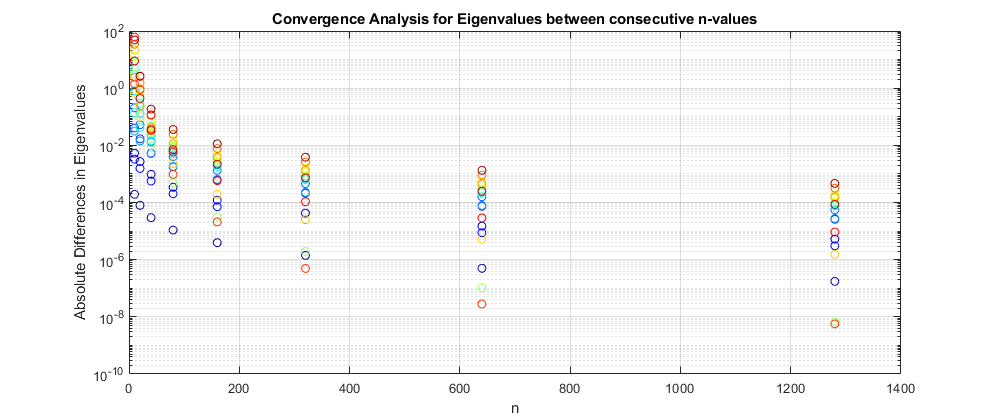
\includegraphics[scale=0.3]{Convergence.png} \\ % Adjust scale as needed
            \footnotesize Rate of convergence of the first 20 eigenvalues for the two-dimensional beam.

            \centering
            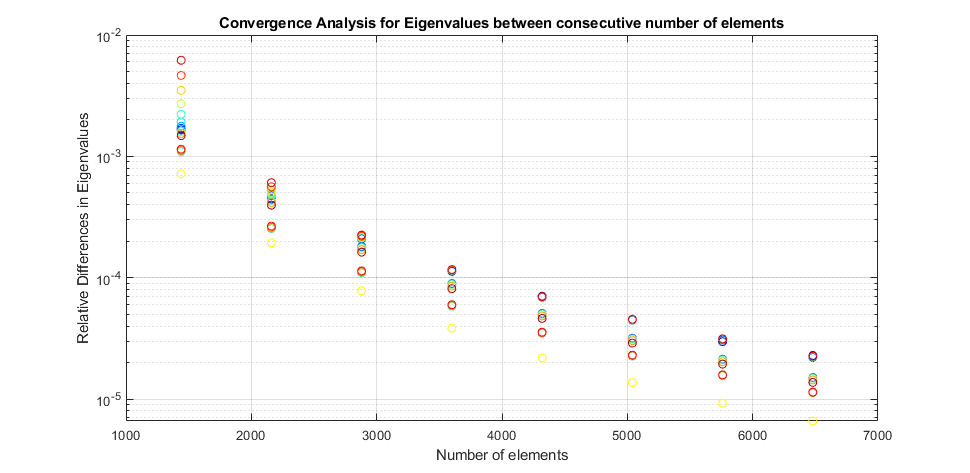
\includegraphics[scale=0.3]{convergence3d.png} \\ % Adjust scale as needed
            \footnotesize Rate of convergence of the first 20 eigenvalues for the three-dimensional beam.
        \end{frame}

\section{Validity of the Timoshenko beam model}
    \begin{frame}{Validity of the Timoshenko beam model}
        \begin{center}
            \begin{minipage}[b]{0.45\linewidth}
                \centering
                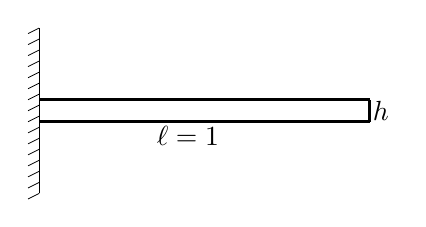
\begin{tikzpicture}[scale=0.7]
                    \draw[line width = 0.4mm] (0,0.2) -- (6,0.2);
                                \draw[line width = 0.4mm] (0,-0.2) -- (6,-0.2);
                                \draw[line width = 0.4mm] (6,-0.2) -- (6,0.2);
                                
                                \node at (6.2,0) {$h$};
                                \node at (2.7,-0.45) {$\ell = 1$};
                                
                                \draw[line width = 0.1mm] (0,-1.5) -- (0,1.5);
                                \draw[line width = 0.1mm] (0,1.5) -- (-0.2,1.4);
                                \draw[line width = 0.1mm] (0,1.3) -- (-0.2,1.2);
                                \draw[line width = 0.1mm] (0,1.1) -- (-0.2,1);
                                \draw[line width = 0.1mm] (0,0.9) -- (-0.2,0.8);
                                \draw[line width = 0.1mm] (0,0.7) -- (-0.2,0.6);
                                \draw[line width = 0.1mm] (0,0.5) -- (-0.2,0.4);
                                \draw[line width = 0.1mm] (0,0.3) -- (-0.2,0.2);
                                \draw[line width = 0.1mm] (0,0.1) -- (-0.2,0);
                                
                                \draw[line width = 0.1mm] (0,-0.1) -- (-0.2,-0.2);
                                \draw[line width = 0.1mm] (0,-0.3) -- (-0.2,-0.4);
                                \draw[line width = 0.1mm] (0,-0.5) -- (-0.2,-0.6);
                                \draw[line width = 0.1mm] (0,-0.7) -- (-0.2,-0.8);
                                \draw[line width = 0.1mm] (0,-0.9) -- (-0.2,-1);
                                \draw[line width = 0.1mm] (0,-1.1) -- (-0.2,-1.2);
                                \draw[line width = 0.1mm] (0,-1.3) -- (-0.2,-1.4);
                                \draw[line width = 0.1mm] (0,-1.5) -- (-0.2,-1.6);
                \end{tikzpicture}
                \captionof{figure}{Two-Dimensional Beam}
            \end{minipage}
            \hfill
            \begin{minipage}[b]{0.45\linewidth}
                \centering
                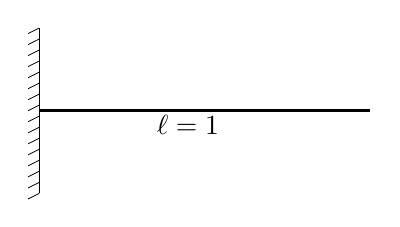
\begin{tikzpicture}[scale=0.7]
                    \draw[line width = 0.4mm] (0,0) -- (6,0);
                            \node at (2.7,-0.25) {$\ell = 1$};
                            
                            \draw[line width = 0.1mm] (0,-1.5) -- (0,1.5);
                            \draw[line width = 0.1mm] (0,1.5) -- (-0.2,1.4);
                            \draw[line width = 0.1mm] (0,1.3) -- (-0.2,1.2);
                            \draw[line width = 0.1mm] (0,1.1) -- (-0.2,1);
                            \draw[line width = 0.1mm] (0,0.9) -- (-0.2,0.8);
                            \draw[line width = 0.1mm] (0,0.7) -- (-0.2,0.6);
                            \draw[line width = 0.1mm] (0,0.5) -- (-0.2,0.4);
                            \draw[line width = 0.1mm] (0,0.3) -- (-0.2,0.2);
                            \draw[line width = 0.1mm] (0,0.1) -- (-0.2,0);
                            
                            \draw[line width = 0.1mm] (0,-0.1) -- (-0.2,-0.2);
                            \draw[line width = 0.1mm] (0,-0.3) -- (-0.2,-0.4);
                            \draw[line width = 0.1mm] (0,-0.5) -- (-0.2,-0.6);
                            \draw[line width = 0.1mm] (0,-0.7) -- (-0.2,-0.8);
                            \draw[line width = 0.1mm] (0,-0.9) -- (-0.2,-1);
                            \draw[line width = 0.1mm] (0,-1.1) -- (-0.2,-1.2);
                            \draw[line width = 0.1mm] (0,-1.3) -- (-0.2,-1.4);
                            \draw[line width = 0.1mm] (0,-1.5) -- (-0.2,-1.6);
                \end{tikzpicture}
                \captionof{figure}{Timoshenko Beam}
            \end{minipage}
        \end{center}
    \end{frame}
    
    \begin{frame}{Comparison of two and three-dimensional models}
        \centering
        \begin{minipage}[b]{0.45\textwidth}
            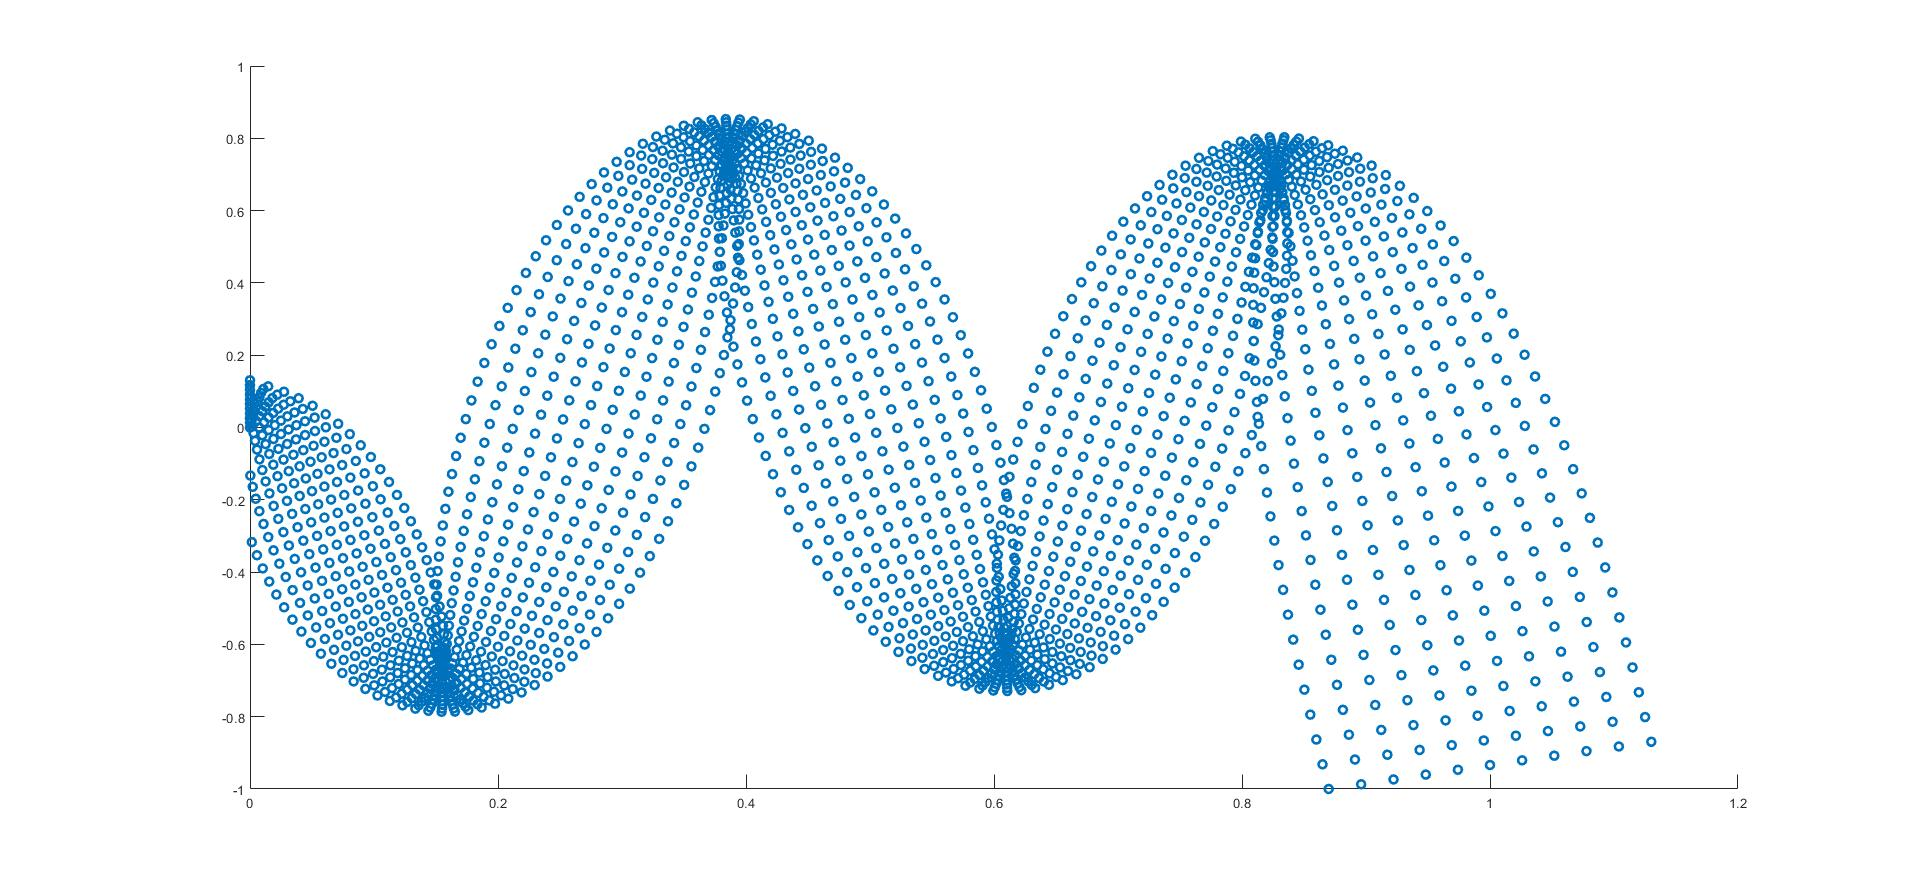
\includegraphics[width=\textwidth]{Beam1.jpg}
            \\ 2D Beam Type - $\lambda_6 = 21.911$
            \label{fig:minipage2}
        \end{minipage}
        \hfill
        \begin{minipage}[b]{0.45\textwidth}
            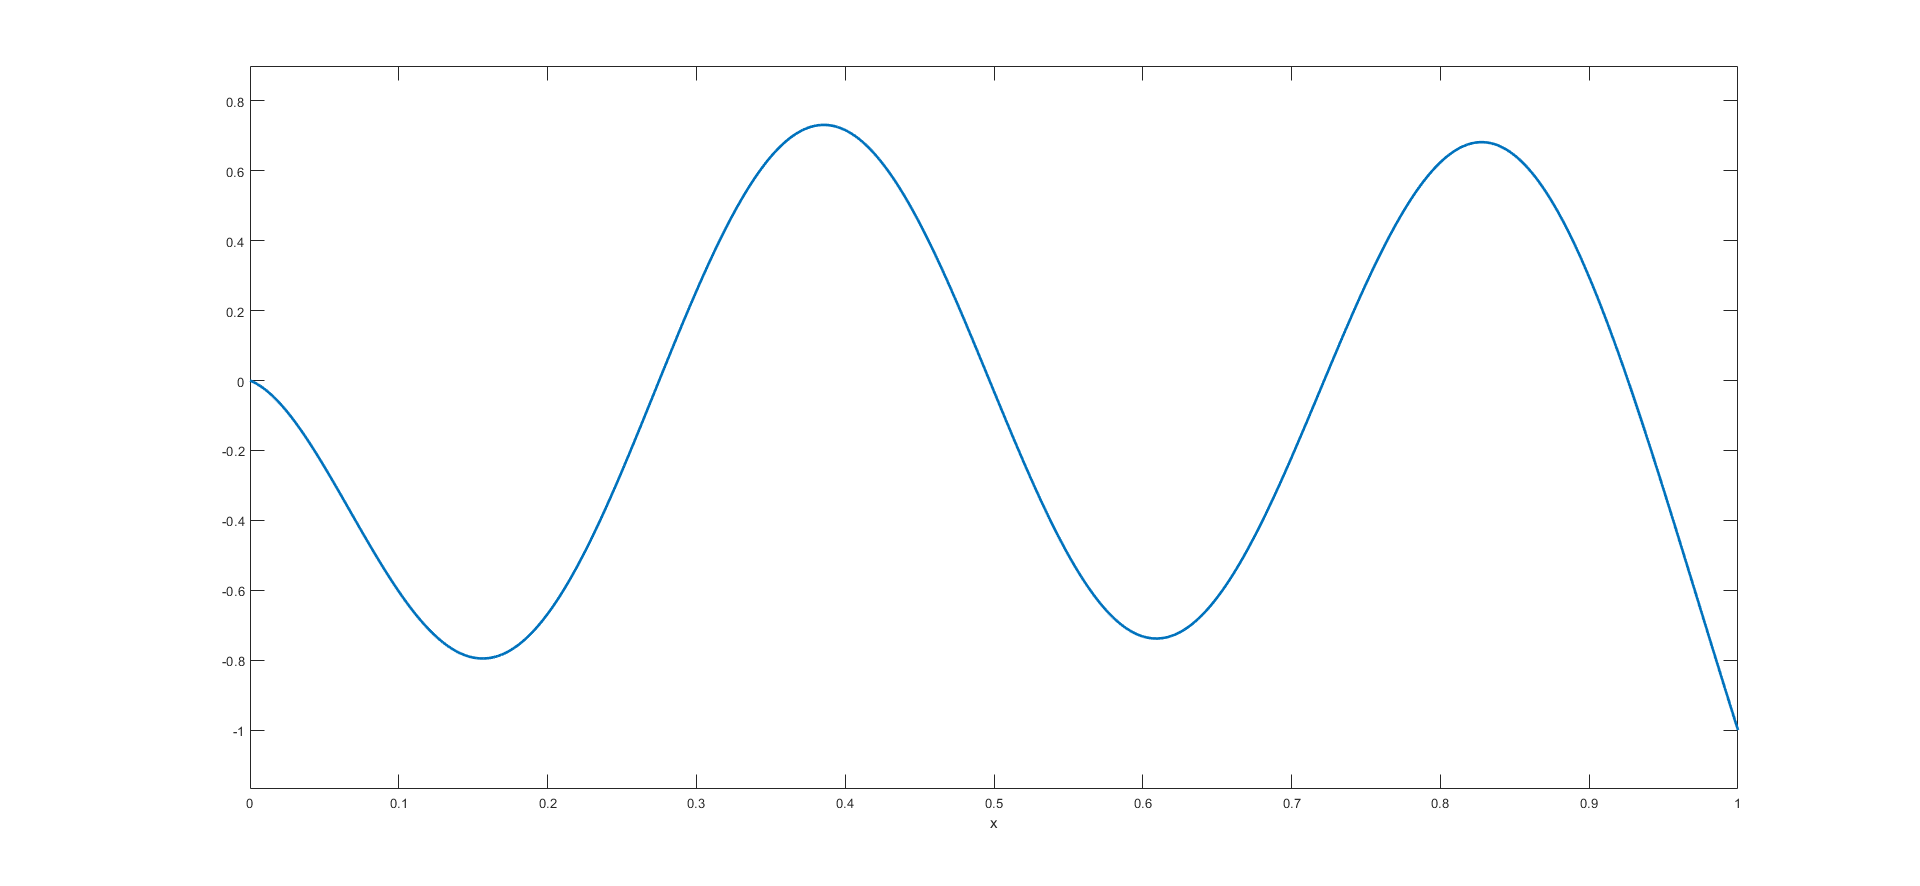
\includegraphics[width=\textwidth]{1DBeam2.png}
            \\ Timoshenko - $\lambda_5 = 21.794$
            \label{fig:minipage1}
        \end{minipage}
        \vspace{1em}
        \begin{minipage}[b]{0.45\textwidth}
            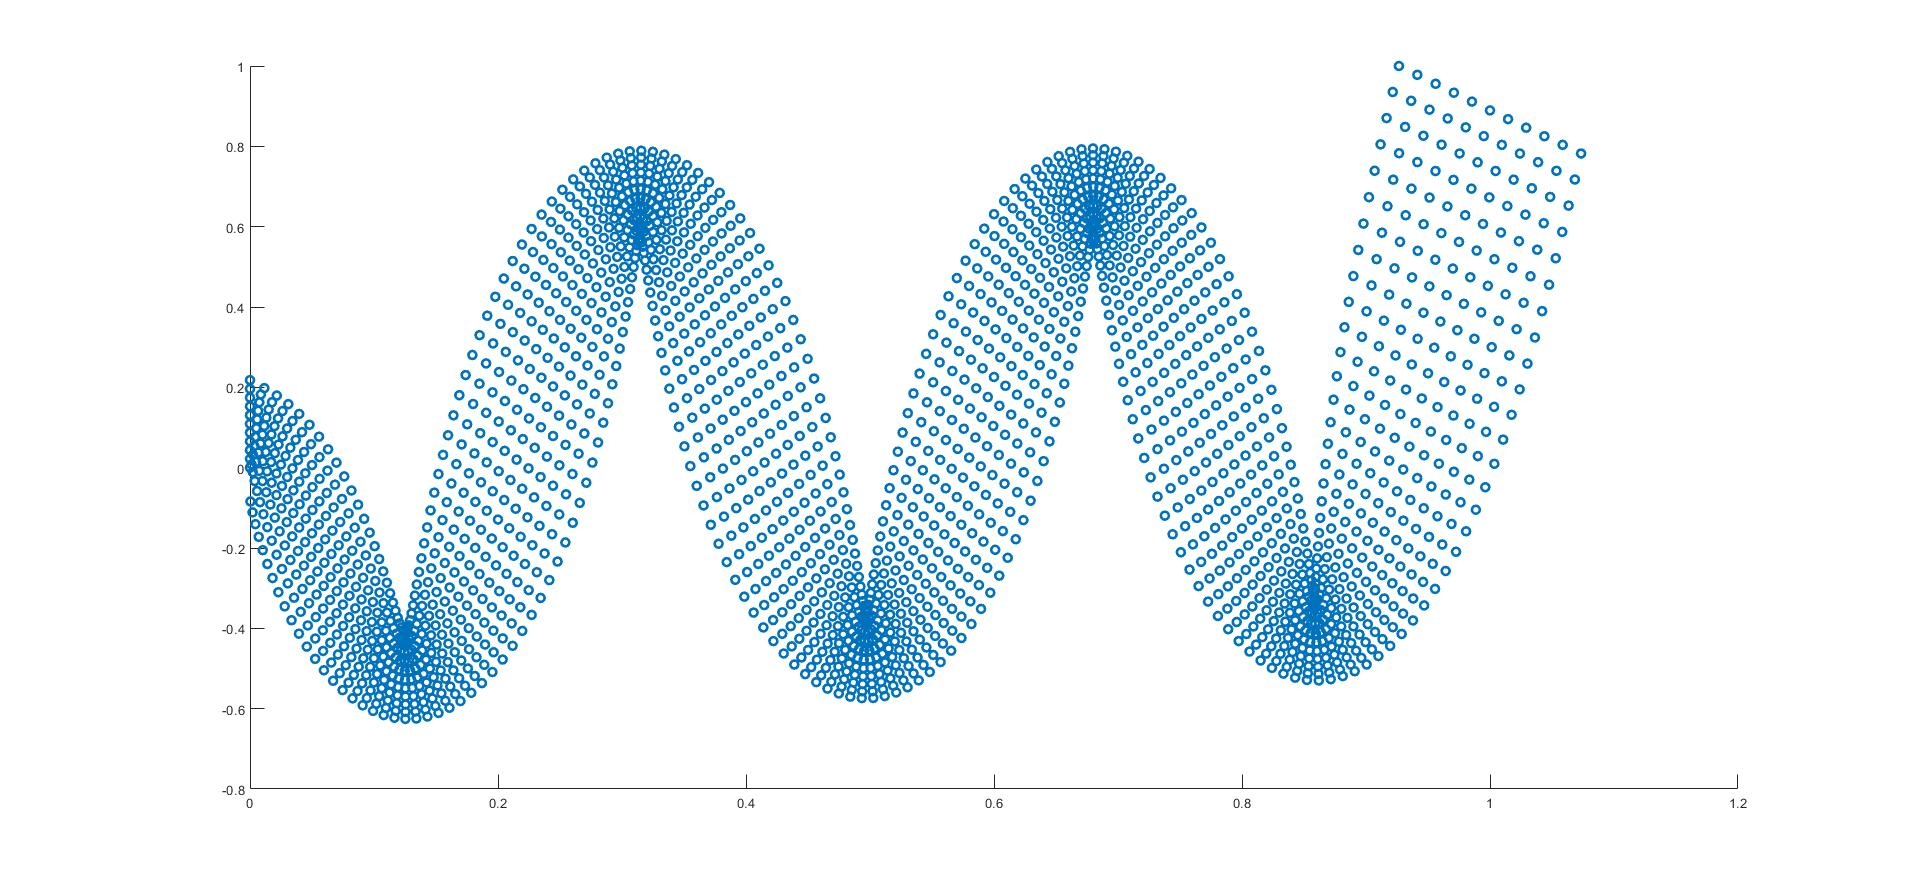
\includegraphics[width=\textwidth]{Beam2.jpg}
            \\ 2D Beam Type - $\lambda_7 = 45.711$
            \label{fig:minipage4}
        \end{minipage}
        \hfill
        \begin{minipage}[b]{0.45\textwidth}
            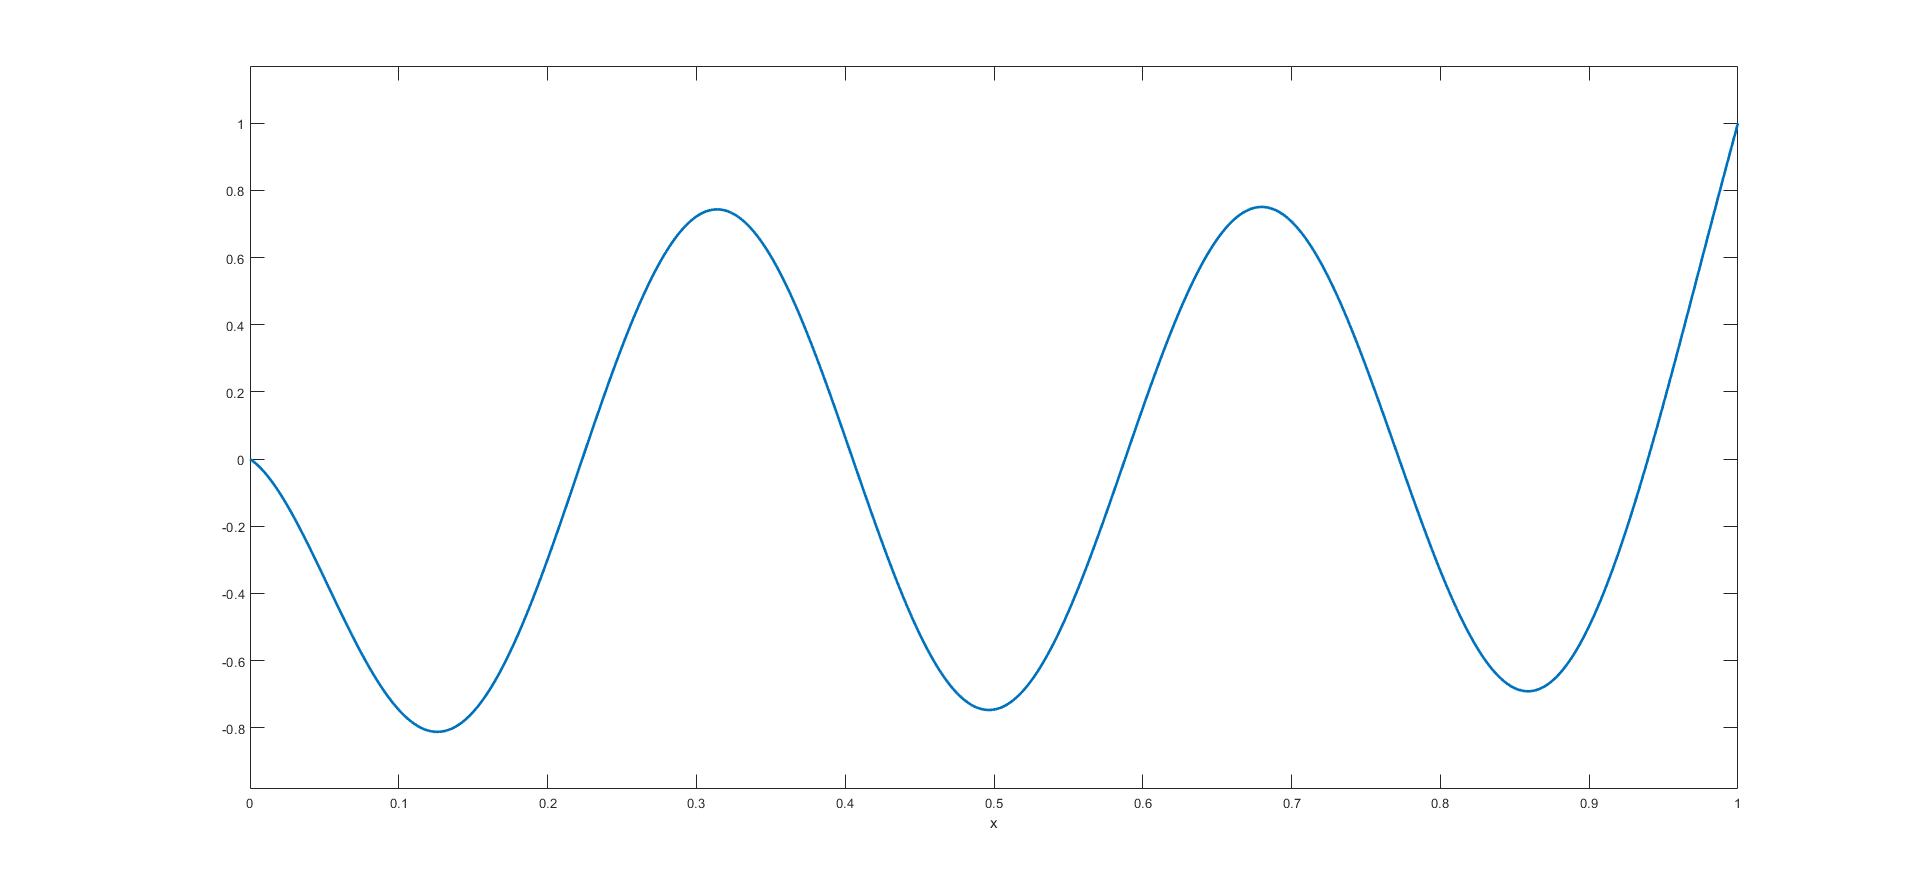
\includegraphics[width=\textwidth]{1DBeam1.png}
            \\ Timoshenko - $\lambda_6 = 45.390$
            \label{fig:minipage3}
        \end{minipage}
        \\ Modal shapes of the displacement $w$ for the beam-type 2D body and the Timoshenko beam with $\alpha = 4800$ ($h = 1/20$).
    \end{frame}
    
    
    \begin{frame}{Comparison of two and three-dimensional models}
        \centering
        \begin{minipage}[b]{0.45\textwidth}
            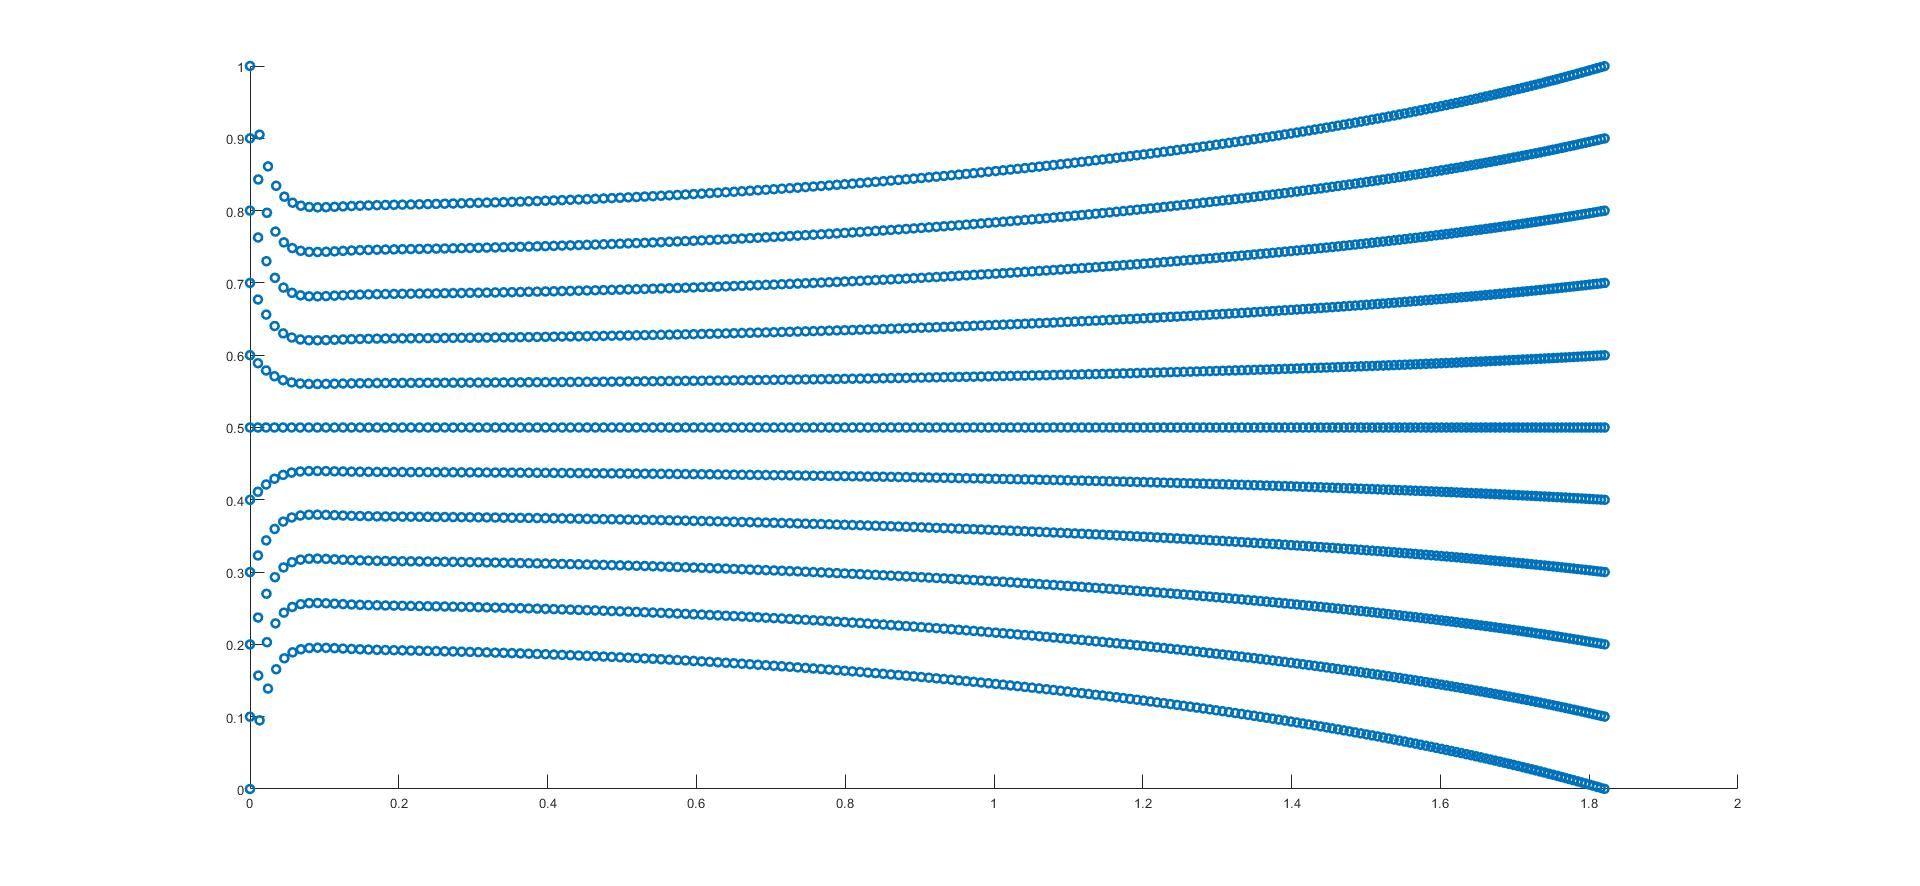
\includegraphics[width=\textwidth]{NotBeam1.jpg}
            \\ Non-Beam Type - $\lambda_4 = 7.7077$
            \label{fig:nonbeam1}
        \end{minipage}
        \hfill
        \begin{minipage}[b]{0.45\textwidth}
            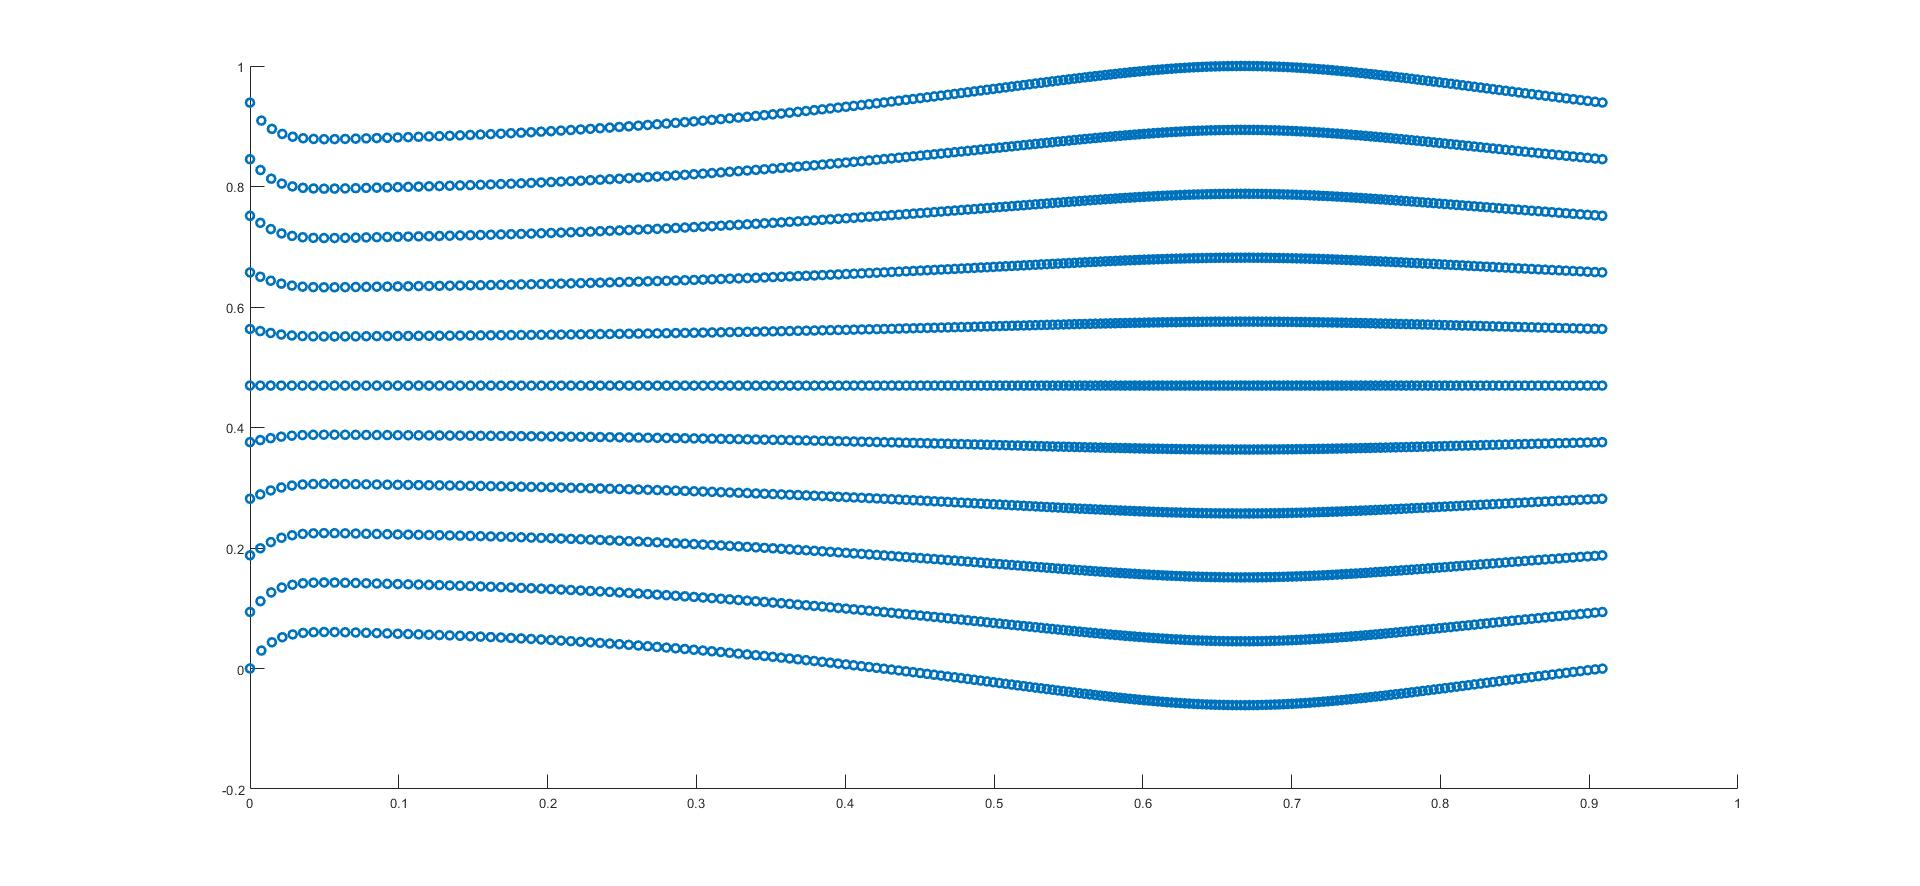
\includegraphics[width=\textwidth]{NotBeam2.jpg}
            \\ Non-Beam Type - $\lambda_8 = 69.344$
            \label{fig:nonbeam2}
        \end{minipage}
        \\ Modal shapes of the displacement $w$ for the non-beam type 2D body with $h = 1/20$.
    \end{frame}
    
    
    \begin{frame}{Comparison of two and three-dimensional models}
        \centering
        \footnotesize
        \renewcommand{\arraystretch}{0.9}
        Results from \cite{LVV09} and results obtained. $0^a$ indicates a 0 due to rounding. Height to lenght ratio of 1 to 10.
    
        \begin{tabular}{cccc|cccc}
            \hline
            & \multicolumn{3}{c}{[LVV09]} & & \multicolumn{3}{c}{Master Dissertation} \\
            
            & 2D & Timo & RE & & 2D & Timo & RE \\
            \hline
            1 & 0.0317 & 0.0316 & 0.00315 & 1 & 0.031713 & 0.031639 & 0.0023407 \\
            2 & 1.14 & 1.14 & $0^a$ & 2 & 1.1413 & 1.1365 & 0.0042050 \\
            3 & 7.72 & - & - & 3 & 7.7161 & - & - \\
            4 & 7.92 & 7.86 & 0.00758 & 4 & 7.918 & 7.8617 & 0.0071116 \\
            5 & 26.2 & 25.9 & 0.0115 & 5 & 26.148 & 25.869 & 0.010669 \\
            6 & 60.8 & 59.9 & 0.0148 & 6 & 60.816 & 59.946 & 0.014303 \\
            7 & 69.3 & - & - & 7 & 69.344 & - & - \\
            8 & 115 & 113 & 0.0174 & 8 & 115.28 & 113.23 & 0.017787 \\
            9 & 192 & 188 & 0.0208 & 9 & 191.57 & 187.55 & 0.020999 \\
            10 & 192 & - & - & 10 & 192.03 & - & - \\
            11 & 291 & 284 & 0.0241 & 11 & 290.76 & 283.81 & 0.023899 \\
            \hline
        \end{tabular}
    
        \footfullcite{LVV09}
    \end{frame}
    
    % \begin{frame}{Eigenvalue problem - FEM}
    %     \centering
    %     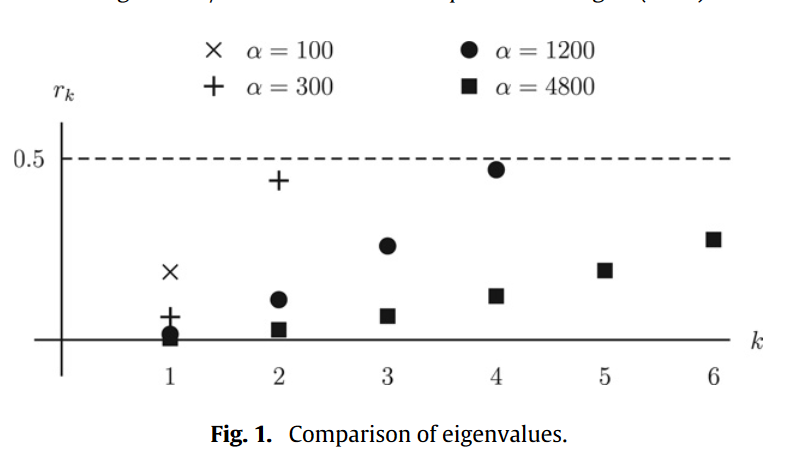
\includegraphics[scale=0.45]{Result.png} \\ % Adjust scale as needed
    %     \footnotesize Rate of convergence of the first 20 eigenvalues.
    %     \label{fig:conv}
    % \end{frame}
    
    \begin{frame}{Comparison of Eigenvalues across Different Parameters}
        \centering
        \footnotesize
        \renewcommand{\arraystretch}{0.8}
        \resizebox{\textwidth}{!}{%
        \begin{tabular}{|cccc||cccc||cccc||cccc|}
            \hline
            \multicolumn{16}{|c|}{Comparison of Eigenvalues} \\
            \hline\hline
            \multicolumn{4}{|c||}{ $h = 1/5$ or $\alpha = 300$} & \multicolumn{4}{c||}{$h =1/10$ or $\alpha = 1200$} & \multicolumn{4}{c||}{$h = 1/20$ or $\alpha = 4800$} & \multicolumn{4}{c|}{$h = 1/30$ or $\alpha = 10800$} \\
            \hline
    
            {i} & {2D} & {j} & {Timo} & {i} & {2D} & {j} & {Timo} & {i} & {2D} & {j} & {Timo} & {i} & {2D} & {j} & {Timo} \\
            \hline
            {1}&0.12151&1&0.12092&1&0.031713&1&0.031639&1&0.008013&1&0.008004&1&0.003568&1&0.003565\\
            {2}&3.5460&2&3.5071&2&1.1413&2     & 1.1365 & 2     & 0.30756 & 2     & 0.30705 & 2     & 0.13869 & 2     & 0.13855 \\
            {3} & {7.7311} &       & {-} & {3}     & {7.7161} &       & {-} & 3     & 2.3273 & 3     & 2.3213 & 3     & 1.0698 & 3     & 1.0683 \\
            {4} & 20.225 & 3     & 19.869 & 4     & 7.9180 & 3     & 7.8617 & {4}     & {7.7077} &       & {-} & 4     & 4.0140 & 4     & 4.0058 \\
            {5} & 56.109 & 4     & 54.766 & 5     & 26.148 & 4     & 25.869 & 5     & 8.5086 & 4     & 8.4762 & {5}     & {7.7047} &       & {-} \\
            {6} & {69.164} &       & {-} & 6     & 60.816 & 5     & 59.946 & 6     & 21.911 & 5     & 21.794 & 6     & 10.655 & 5     & 10.625 \\
            {7} & 114.03 & 5     & 110.75 & {7}     & {69.344} &       & {-} & 7     & 45.711 & 6     & 45.390 & 7     & 22.975 & 6     & 22.890 \\
            {8} & {189.17} &  6     & {186.50} & 8     & 115.28 & 6     & 113.23 & {8}     & {69.344} &       & {-} & 8     & 43.113 & 7     & 42.909 \\
            {9} & {192.61} &      &  & {9}     & {191.57} &   7  & {187.55} & 9     & 82.887 & 7     & 82.154 & {9}     & {69.331} &       & {-} \\
            {10} & 285.85 & 7     & 277.64 & {10}    & {192.03} &      & {-} & 10    & 136.03 & 8     & 134.58 & 10    & 73.230 & 8     & 72.803 \\
            {11} & 328.40 & 8     & 330.29 & 11    & 290.76 & 8     & 283.81 & {11}    & {192.48} &       & {-} & 11    & 115.41 & 9     & 114.61 \\
            {12} & {357.08} &       & {-} & {12}    & {374.45} &       & {-} & 12    & 207.29 & 9     & 204.69 & 12    & 171.61 & 10    & 170.20 \\
            {13} & 397.33 & 9     & 394.02 & 13    & 413.20 & 9     & 402.27 & 13    & 298.38 & 10    & 294.10 & {13}    & {192.52} &       & {-} \\
            {14} & 442.00   & 10    & 439.52 & 14    & 558.67 & 10    & 542.65 & {14}    & {376.83} &       & {-} & 14    & 243.56 & 11    & 241.26 \\
            {15} & {533.71} &       & {-} & {15}    & {614.11} &       & {-} & 15    & 410.63 & 11    & 404.01 & 15    & 332.83 & 12    & 329.28 \\
            {16} & 538.97 & 11    & 541.55 & 16    & 726.26 & 11    & 704.15 & 16    & 545.03 & 12    & 535.32 & {16}    & {377.16} &       & {-} \\
            {17} & {596.06} &       & {-} & {17}    & {906.28} &       & {-} & {17}    & {621.95} &       & {-} & 17    & 440.77 & 13    & 435.51 \\
            {18} & 602.77 & 12    & 596.09 & 18    & 913.69 & 12    & 884.92 & 18    & 702.30 & 13    & 688.64 & 18    & 568.51 & 14    & 561.04 \\
            {19} & {657.87} &       & {-} & 19    & 1113.7 & 13    & 1080.1 & 19    & 882.95 & 14    & 864.40 & {19}    & {623.05} &       & {-} \\
            {20} & 717.37 & 13    & 731.74 & {20}    & {1218.0}  &       & {-} & {20}    & {927.18} &       & {-} & 20    & 717.04 & 15    & 706.74 \\
            \hline
            \multicolumn{2}{|c}{Max RE:} & \multicolumn{2}{c||}{3.1718\%} & \multicolumn{2}{c}{Max RE:} & \multicolumn{2}{c||}{3.1486\%} & \multicolumn{2}{c}{Max RE:} & \multicolumn{2}{c||}{2.1018\%} & \multicolumn{2}{c}{Max RE:} & \multicolumn{2}{c|}{1.4361\%} \\
            \hline
        \end{tabular}}
    \end{frame}
        
\section{Validity of the Two-dimensional beam model}
    \begin{frame}{Validity of the Two-dimensional beam model}
        \begin{center}
            \begin{minipage}[b]{0.45\linewidth}
                \centering
                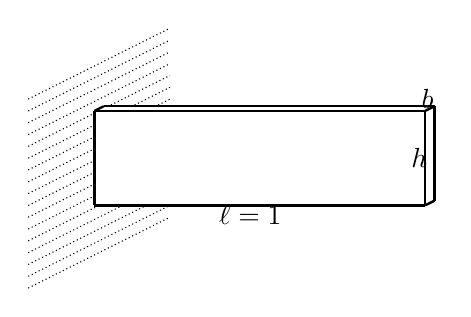
\begin{tikzpicture}[scale=0.6]
                    \draw[line width = 0.3mm] (-0.1,1) -- (6.9,1);
                    \draw[line width = 0.3mm] (-0.1,-1) -- (6.9,-1);
                    \draw[line width = 0.3mm] (6.9,-1) -- (6.9,1);
                    \draw[line width = 0.3mm] (-0.1,-1) -- (-0.1,1);
                    
                    \draw[line width = 0.3mm] (0.1,1.1) -- (7.1,1.1);
                    \draw[line width = 0.3mm] (7.1,-0.9) -- (7.1,1.1);
                    
                    \draw[line width = 0.3mm] (-0.1,1) -- (0.1,1.1);
                    \draw[line width = 0.3mm] (6.9,1) -- (7.1,1.1);
                    \draw[line width = 0.3mm] (6.9,-1) -- (7.1,-0.9);
                    
                    
                    
                    \draw[scale=0.5, domain=-3:3, smooth, variable=\x,densely dotted] plot ({\x}, {0.5*\x+4});
                    \draw[scale=0.5, domain=-3:3, smooth, variable=\x,densely dotted] plot ({\x}, {0.5*\x+3.5});
                    \draw[scale=0.5, domain=-3:3, smooth, variable=\x,densely dotted] plot ({\x}, {0.5*\x+3});
                    \draw[scale=0.5, domain=-3:3, smooth, variable=\x,densely dotted] plot ({\x}, {0.5*\x+2.5});
                    
                    \draw[scale=0.5, domain=-3:-0.1, smooth, variable=\x,densely dotted] plot ({\x}, {0.5*\x+2});
                    \draw[scale=0.5, domain=-3:-0.1, smooth, variable=\x,densely dotted] plot ({\x}, {0.5*\x+1.5});
                    \draw[scale=0.5, domain=-3:-0.1, smooth, variable=\x,densely dotted] plot ({\x}, {0.5*\x+1});
                    
                    \draw[scale=0.5, domain=0.5:3, smooth, variable=\x,densely dotted] plot ({\x}, {0.5*\x+2});
                    \draw[scale=0.5, domain=1.5:3, smooth, variable=\x,densely dotted] plot ({\x}, {0.5*\x+1.5});
                    \draw[scale=0.5, domain=2.5:3, smooth, variable=\x,densely dotted] plot ({\x}, {0.5*\x+1});
                    
                    \draw[scale=0.5, domain=-3:-0.1, smooth, variable=\x,densely dotted] plot ({\x}, {0.5*\x+0.5});
                    \draw[scale=0.5, domain=-3:-0.1, smooth, variable=\x,densely dotted] plot ({\x}, {0.5*\x});
                    \draw[scale=0.5, domain=-3:-0.1, smooth, variable=\x,densely dotted] plot ({\x}, {0.5*\x-0.5});
                    \draw[scale=0.5, domain=-3:-0.1, smooth, variable=\x,densely dotted] plot ({\x}, {0.5*\x-1});
                    \draw[scale=0.5, domain=-3:-0.1, smooth, variable=\x,densely dotted] plot ({\x}, {0.5*\x-1.5});
                    \draw[scale=0.5, domain=-3:0, smooth, variable=\x,densely dotted] plot ({\x}, {0.5*\x-2});
                    \draw[scale=0.5, domain=-3:1, smooth, variable=\x,densely dotted] plot ({\x}, {0.5*\x-2.5});
                    \draw[scale=0.5, domain=-3:2, smooth, variable=\x,densely dotted] plot ({\x}, {0.5*\x-3});
                    \draw[scale=0.5, domain=-3:3, smooth, variable=\x,densely dotted] plot ({\x}, {0.5*\x-3.5});
                    \draw[scale=0.5, domain=-3:3, smooth, variable=\x,densely dotted] plot ({\x}, {0.5*\x-4});
                    
                    \node at (6.95,1.25) {$b$};
                    \node at (6.78,0) {$h$};
                    \node at (3.2,-1.2) {$\ell = 1$};
                \end{tikzpicture}
                \captionof{figure}{Three-Dimensional Beam}
            \end{minipage}
            \hfill
            \begin{minipage}[b]{0.45\linewidth}
                \centering
                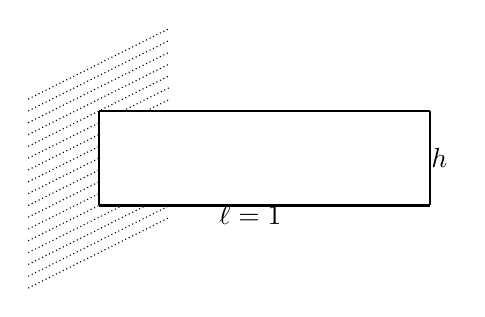
\begin{tikzpicture}[scale=0.6]
                    \draw[line width = 0.3mm] (0,1) -- (7,1);~
                    \draw[line width = 0.3mm] (0,-1) -- (7,-1);
                    \draw[line width = 0.3mm] (7,-1) -- (7,1);
                    \draw[line width = 0.3mm] (0,-1) -- (0,1);
                    
                    
                    \draw[scale=0.5, domain=-3:3, smooth, variable=\x,densely dotted] plot ({\x}, {0.5*\x+4});
                    \draw[scale=0.5, domain=-3:3, smooth, variable=\x,densely dotted] plot ({\x}, {0.5*\x+3.5});
                    \draw[scale=0.5, domain=-3:3, smooth, variable=\x,densely dotted] plot ({\x}, {0.5*\x+3});
                    \draw[scale=0.5, domain=-3:3, smooth, variable=\x,densely dotted] plot ({\x}, {0.5*\x+2.5});
                    \draw[scale=0.5, domain=-3:3, smooth, variable=\x,densely dotted] plot ({\x}, {0.5*\x+2});
                    
                    \draw[scale=0.5, domain=-3:0, smooth, variable=\x,densely dotted] plot ({\x}, {0.5*\x+1.5});
                    \draw[scale=0.5, domain=-3:0, smooth, variable=\x,densely dotted] plot ({\x}, {0.5*\x+1});
                    
                    
                    \draw[scale=0.5, domain=1:3, smooth, variable=\x,densely dotted] plot ({\x}, {0.5*\x+1.5});
                    \draw[scale=0.5, domain=2:3, smooth, variable=\x,densely dotted] plot ({\x}, {0.5*\x+1});
                    
                    \draw[scale=0.5, domain=-3:0, smooth, variable=\x,densely dotted] plot ({\x}, {0.5*\x+0.5});
                    \draw[scale=0.5, domain=-3:0, smooth, variable=\x,densely dotted] plot ({\x}, {0.5*\x});
                    \draw[scale=0.5, domain=-3:0, smooth, variable=\x,densely dotted] plot ({\x}, {0.5*\x-0.5});
                    \draw[scale=0.5, domain=-3:0, smooth, variable=\x,densely dotted] plot ({\x}, {0.5*\x-1});
                    \draw[scale=0.5, domain=-3:0, smooth, variable=\x,densely dotted] plot ({\x}, {0.5*\x-1.5});
                    \draw[scale=0.5, domain=-3:0, smooth, variable=\x,densely dotted] plot ({\x}, {0.5*\x-2});
                    \draw[scale=0.5, domain=-3:1, smooth, variable=\x,densely dotted] plot ({\x}, {0.5*\x-2.5});
                    \draw[scale=0.5, domain=-3:2, smooth, variable=\x,densely dotted] plot ({\x}, {0.5*\x-3});
                    \draw[scale=0.5, domain=-3:3, smooth, variable=\x,densely dotted] plot ({\x}, {0.5*\x-3.5});
                    \draw[scale=0.5, domain=-3:3, smooth, variable=\x,densely dotted] plot ({\x}, {0.5*\x-4});
                    
                    \node at (7.2,0) {$h$};
                    \node at (3.2,-1.2) {$\ell = 1$};
                \end{tikzpicture}
                \captionof{figure}{Two-dimensional Beam}
            \end{minipage}
        \end{center}
    \end{frame}

    \begin{frame}{Three-Dimensional model vs Two-Dimensional model}
        \centering
        \begin{minipage}[b]{0.45\textwidth}
            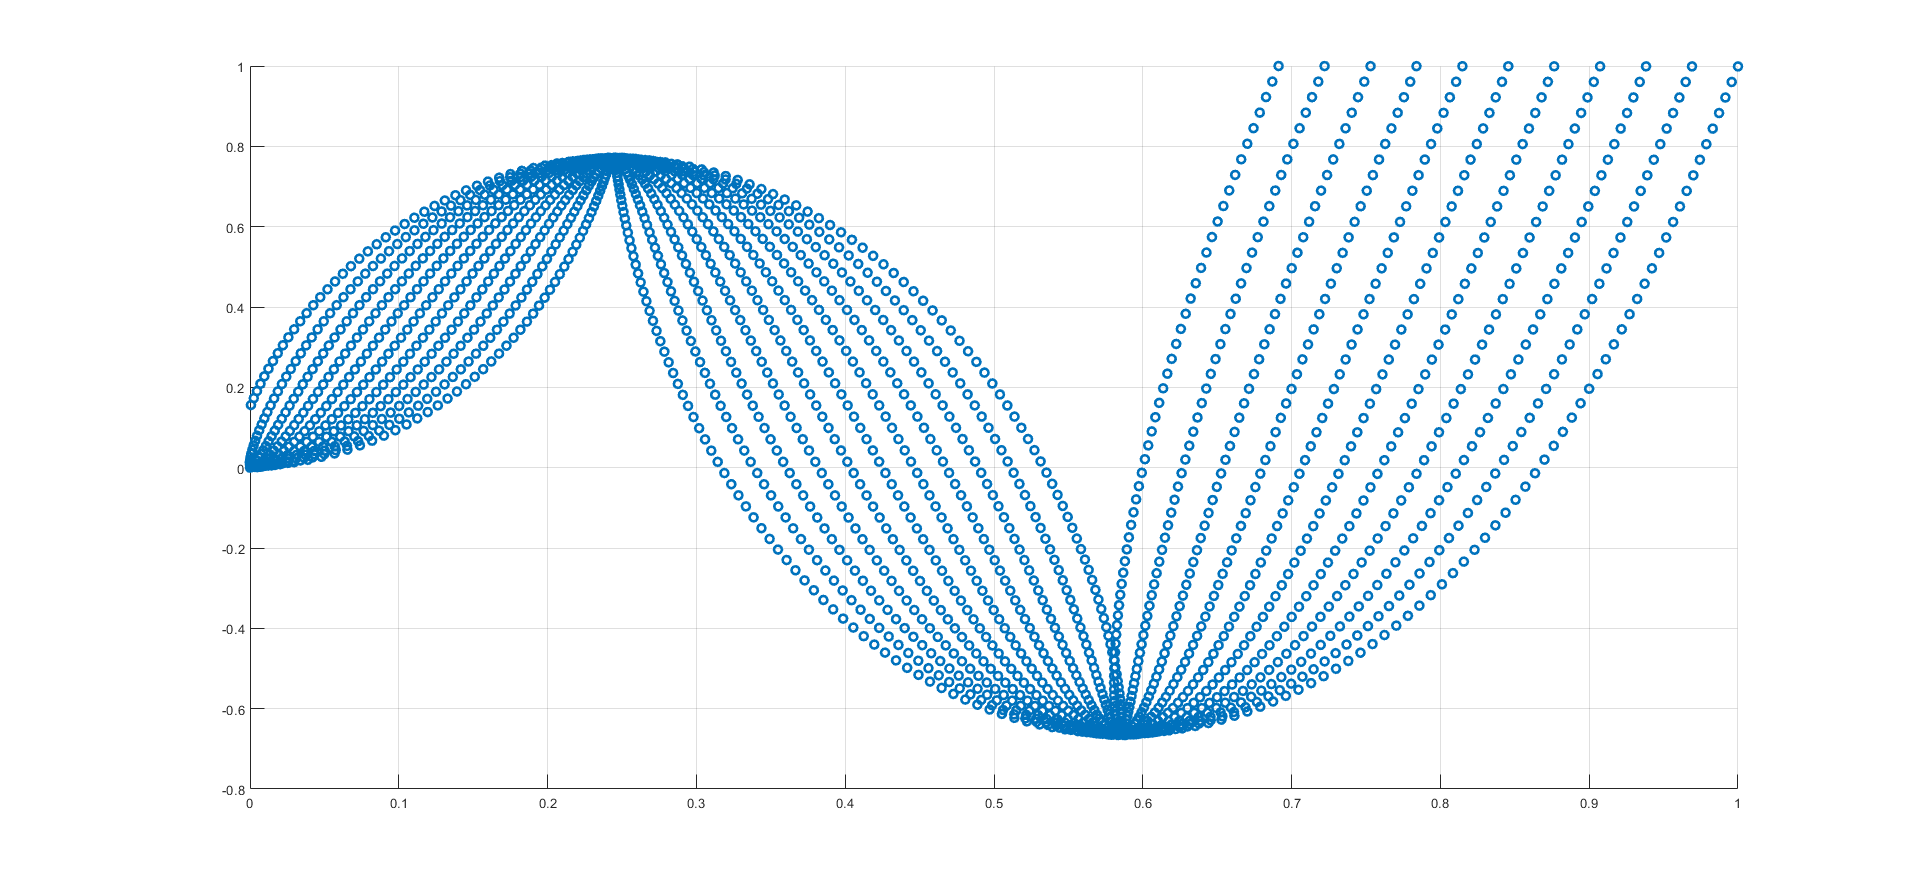
\includegraphics[width=\textwidth]{3D12.png}
            \\ 3D Beam Type - $\lambda_{12} = 2.3293$
            \label{fig:minipage2}
        \end{minipage}
        \hfill
        \begin{minipage}[b]{0.45\textwidth}
            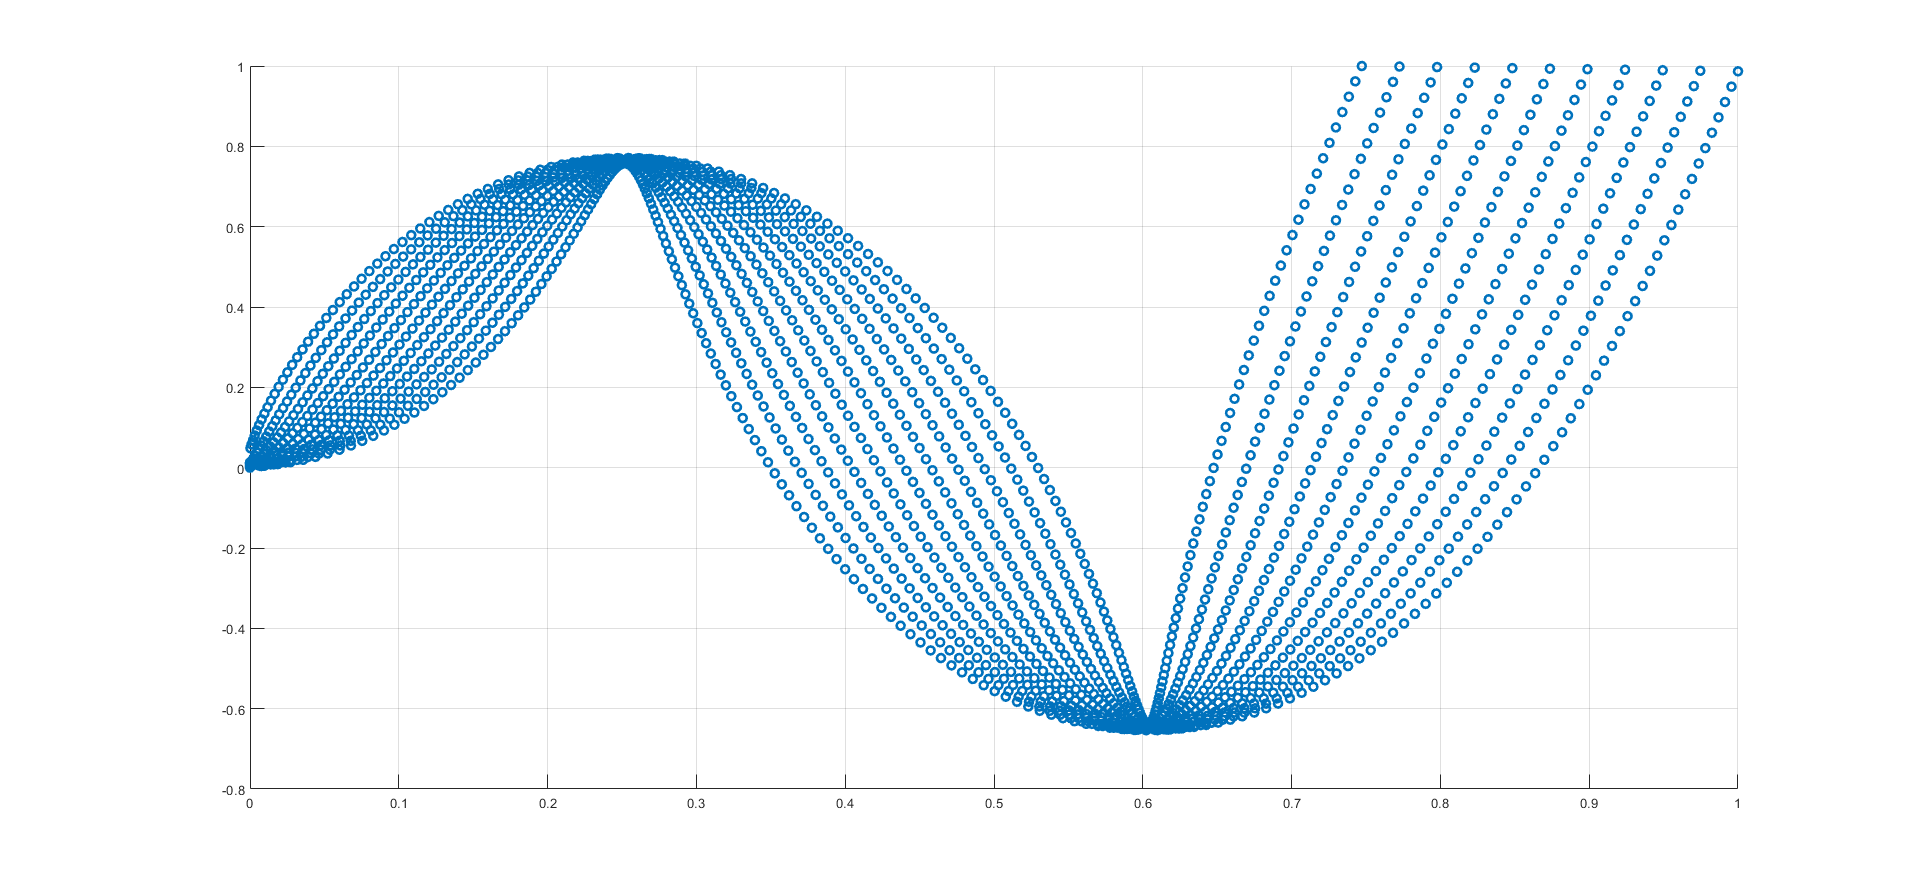
\includegraphics[width=\textwidth]{2D3.png}
            \\ 2D Beam Type - $\lambda_3 = 2.3273$
            \label{fig:minipage1}
        \end{minipage}
    
        \vspace{1em} % spacing between the rows
    
        \begin{minipage}[b]{0.45\textwidth}
            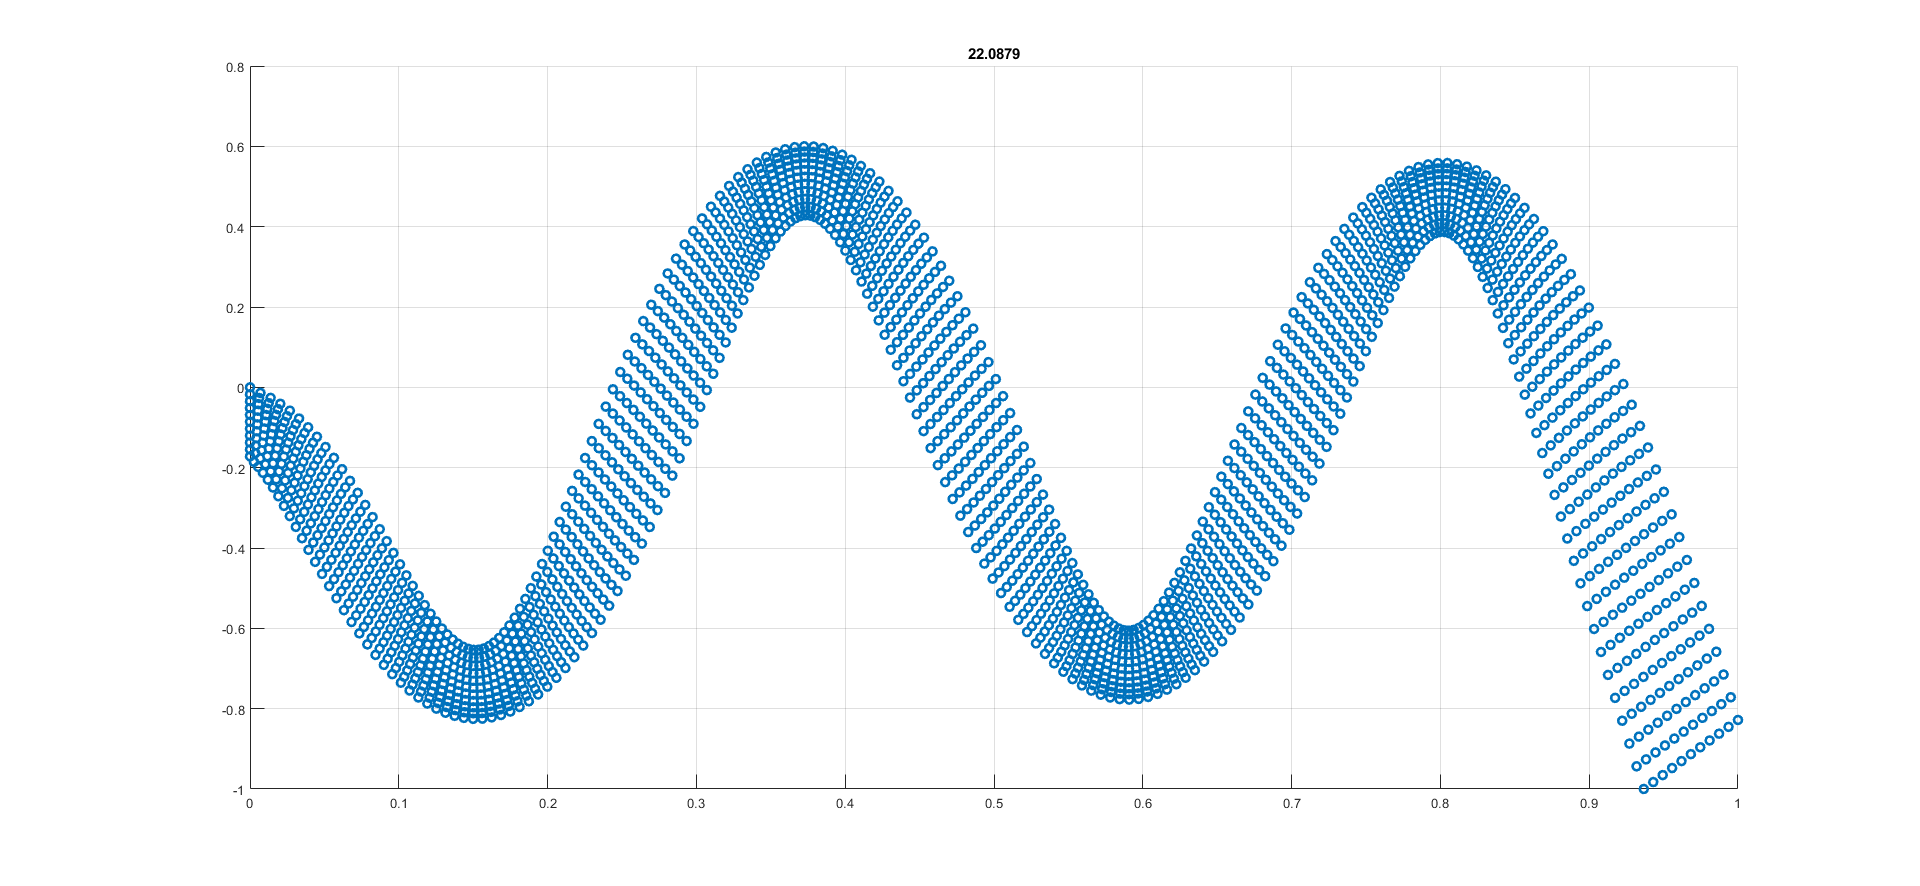
\includegraphics[width=\textwidth]{3D22.png}
            \\ 3D Beam Type - $\lambda_{24} = 21.929$
            \label{fig:minipage4}
        \end{minipage}
        \hfill
        \begin{minipage}[b]{0.45\textwidth}
            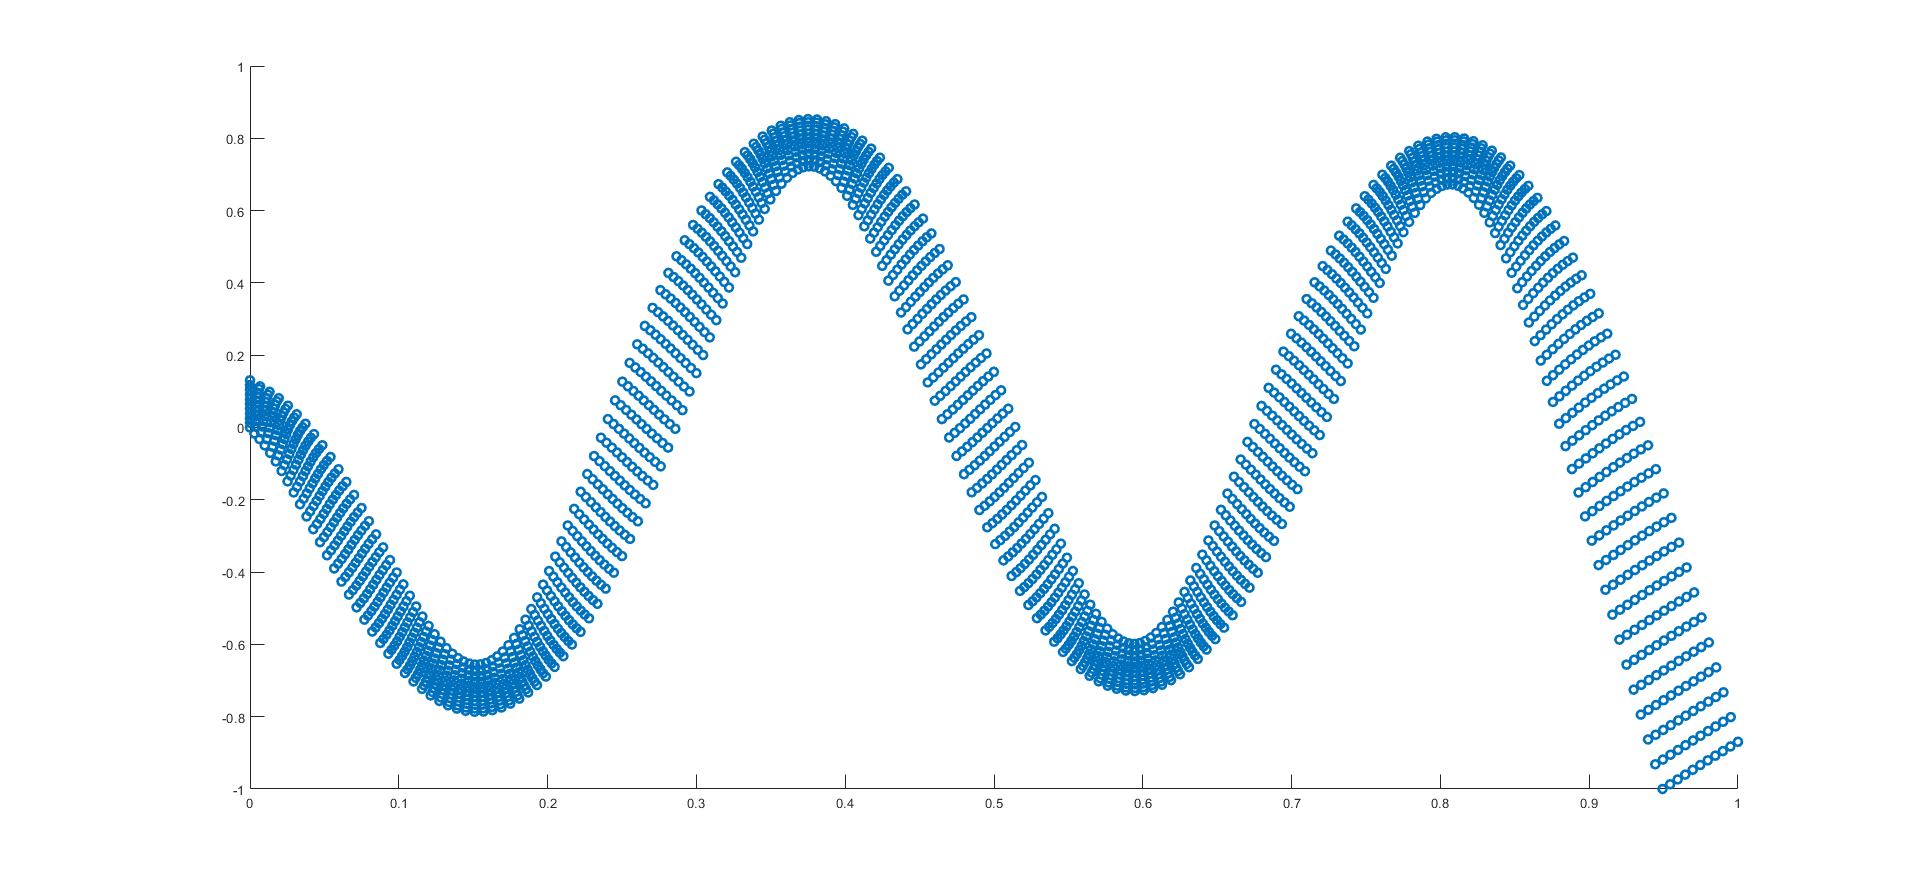
\includegraphics[width=\textwidth]{2D6.png}
            \\ 2D Beam Type - $\lambda_6 = 21.911$
            \label{fig:minipage3}
        \end{minipage}
    
        Mode shapes of the displacement \( w \) with \( h=1/20 \).
    
    \end{frame}
    
    \begin{frame}{Three-Dimensional model}
        \centering
        \begin{minipage}[b]{0.45\textwidth}
            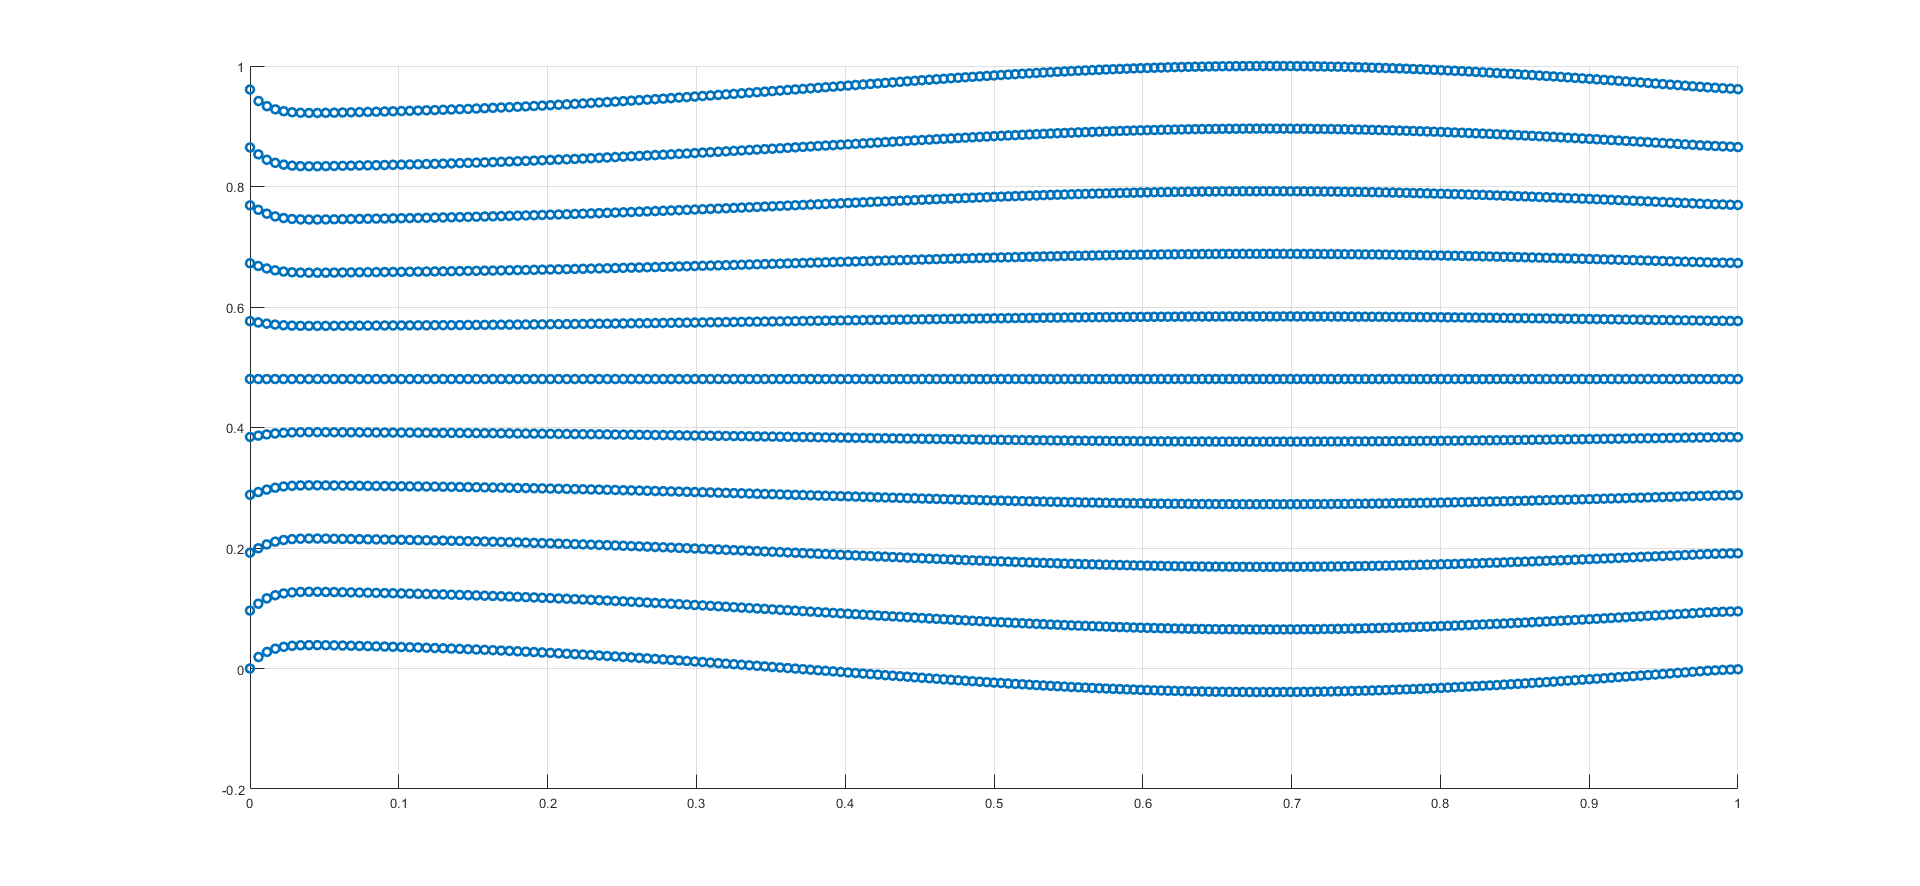
\includegraphics[width=\textwidth]{3D33.png}
            \\ 3D Non-Beam Type - $\lambda_{33} = 69.374$
            \label{fig:minipage6}
        \end{minipage}
        \hfill
        \begin{minipage}[b]{0.45\textwidth}
            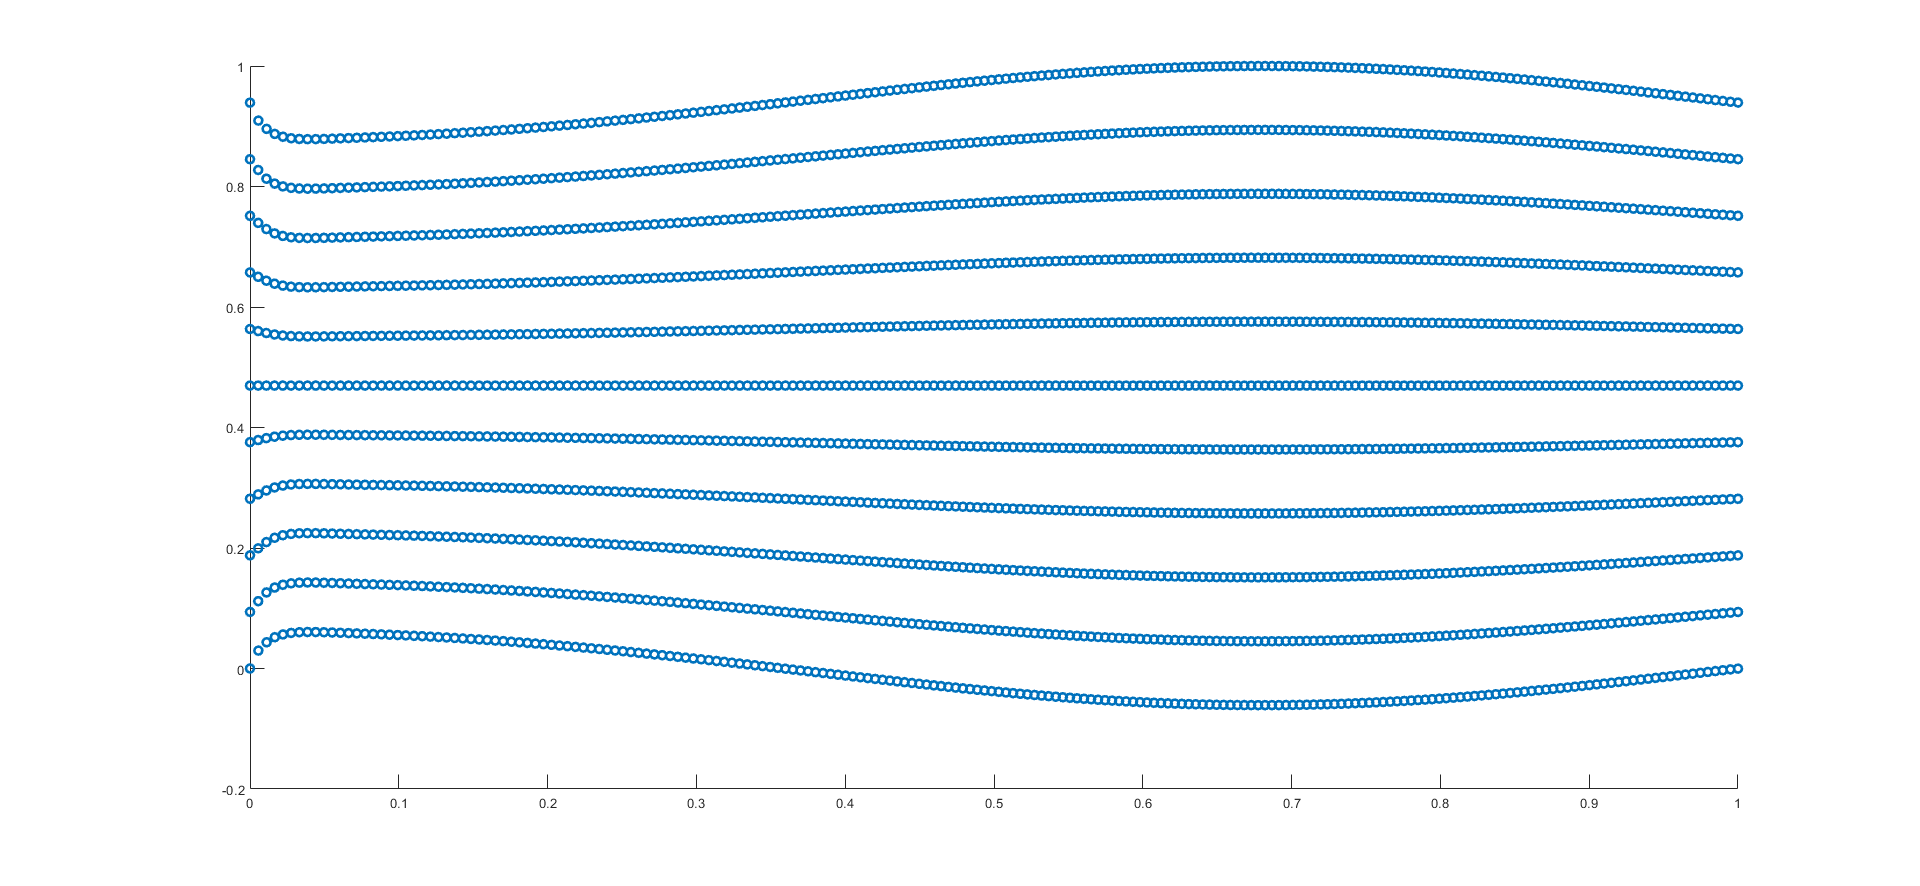
\includegraphics[width=\textwidth]{2D8.png}
            \\ 2D Non-Beam Type - $\lambda_8 = 69.344$
            \label{fig:minipage5}
        \end{minipage}
    
        \vspace{1em} % spacing between the rows
    
        \begin{minipage}[b]{0.45\textwidth}
            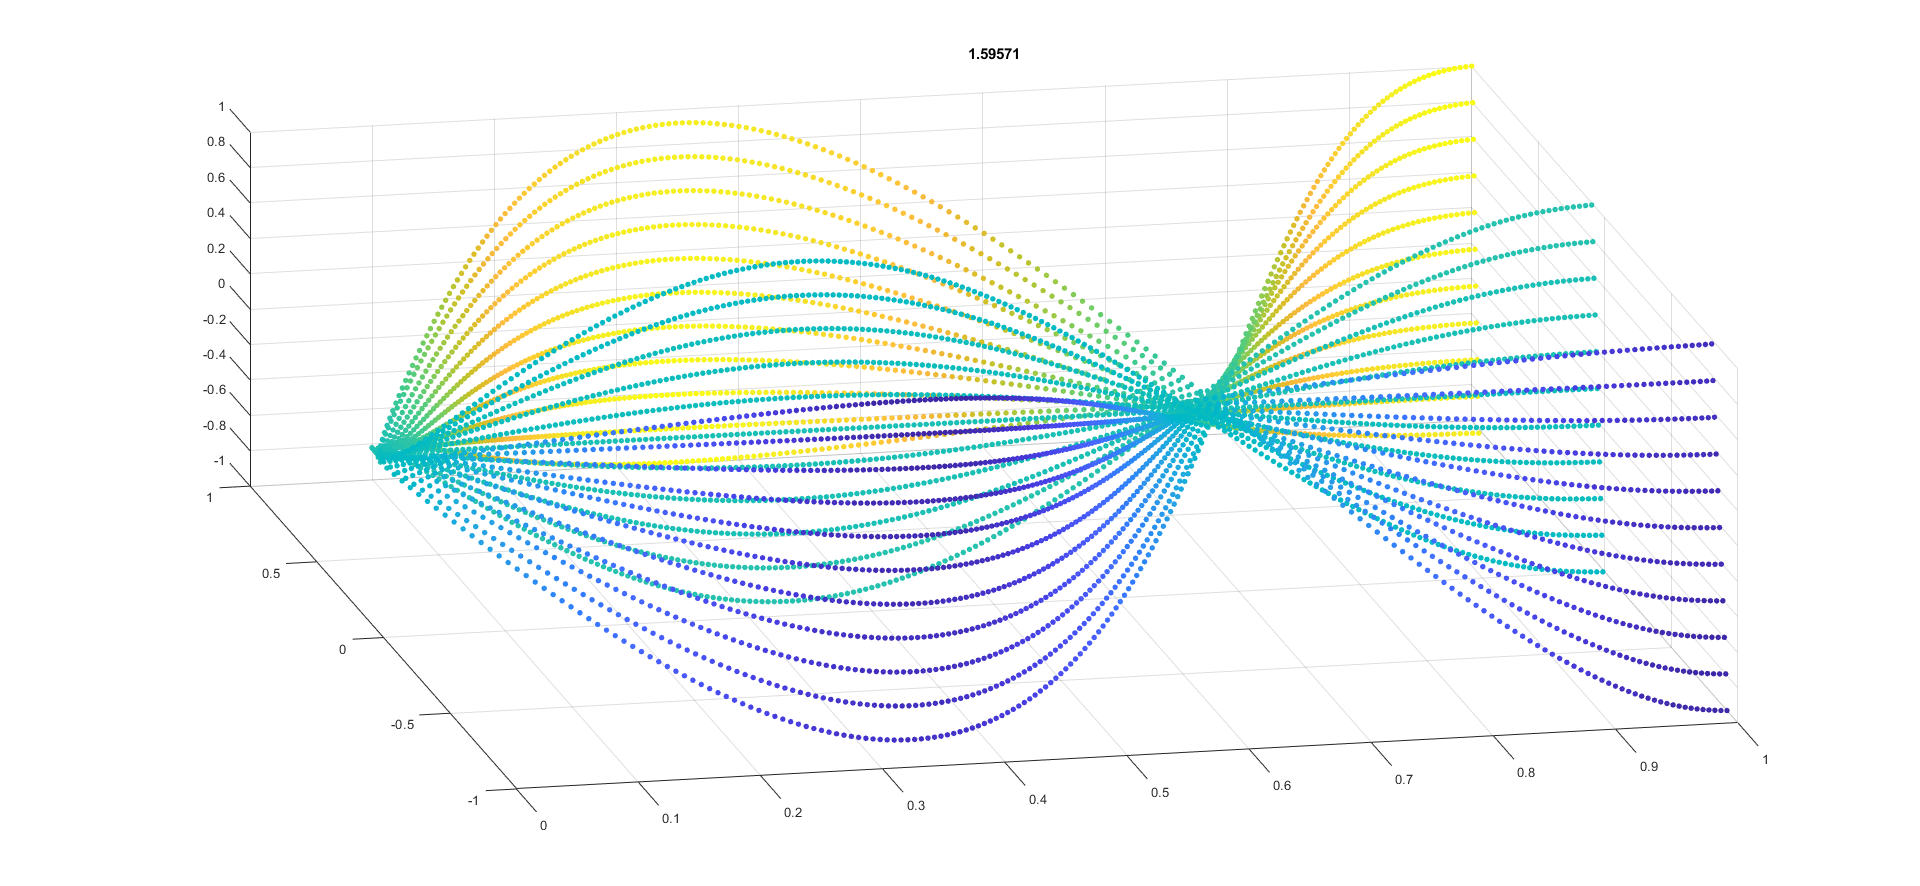
\includegraphics[width=\textwidth]{3DNonBeam10.png}
            \\ Non-2D Type - $\lambda_{10}$
            \label{fig:minipage8}
        \end{minipage}
        \hfill
        \begin{minipage}[b]{0.45\textwidth}
            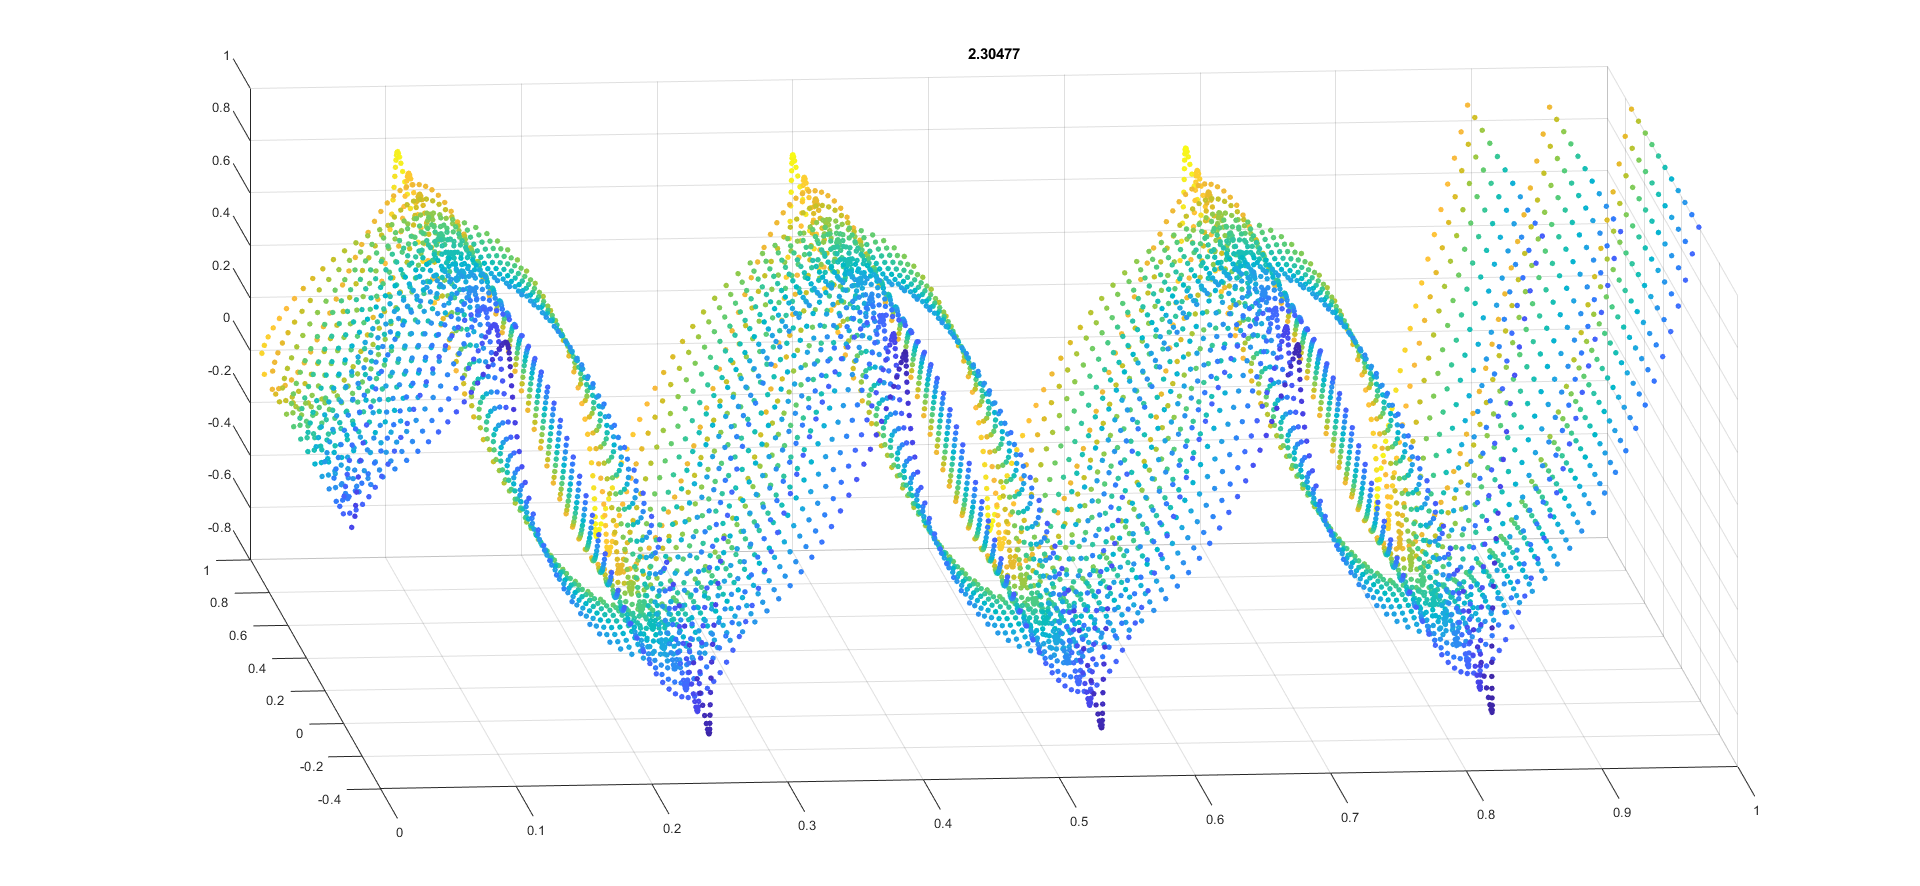
\includegraphics[width=\textwidth]{3DNonBeam11.png}
            \\ Non-2D Type - $\lambda_{11}$
            \label{fig:minipage7}
        \end{minipage}
    
        Mode shapes of the displacement \( w \) with \( \alpha = 4800 \).
    \end{frame}

    \begin{frame}
        \begin{table}[htbp]
            \scalebox{.8}{
            \makebox[\textwidth]{
                \begin{tabular}{|cc|cc|cc|cc||cc|}
                    \hline
                    \multicolumn{10}{|c|}{{Comparsion of Eigenvalues with $h = 1/5$, with decreasing $b$ and $b < h$.} \\
                    \hline
                    \hline
                    i     & {b = h} & i     & {b = 1/2 h} & i     & {b = 1/4 h} & i     & {b = 1/8 h} & j     & 2D \\
                    \hline
                    {2} & 0.12307 & {2} & 0.12234 & {2} & 0.12198 & {3} & 0.12178 & 1     & 0.12151 \\
                    {3} & 3.5773 & {5} & 3.5630 & {6} & 3.5558 & {8} & 3.5519 & 2     & 3.5460 \\
                    \rowcolor{lightgray}{5} & 7.7799 & {6} & 7.7596 & {8} & 7.7471 & {11} & 7.7401 & 3     & 7.7311 \\
                    {8} & 20.334 & {9} & 20.283 & {11} & 20.26 & {14} & 20.247 & 4     & 20.225 \\
                    {10} & 56.247 & {12} & 56.173 & {15} & 56.156 & {22} & 56.142 & 5     & 56.109 \\
                    \rowcolor{lightgray}{11} & 69.197 & {14} & 69.319 & {17} & 69.281 & {24} & 69.238 & 6     & 69.164 \\
                    {14} & 114.03 & {16} & 114.01 & {20} & 114.05 & {29} & 114.06 & 7     & 114.03 \\
                    \rowcolor{lightgray}{17} & 187.01 & {19} & 189.14 & {25} & 189.37 & {36} & 189.34 & 8     & 189.17 \\
                    {18} & 192.21 & {20} & 192.41 & {26} & 192.58 & {37} & 192.63 & 9     & 192.61 \\
                    {21} & 284.76 & {23} & 285.43 & {31} & 285.74 & {42} & 285.84 & 10    & 285.85 \\
                    {23} & 327.57 & {26} & 328.24 & {35} & 328.37 & {46} & 328.40 & 11    & 328.40 \\
                    \rowcolor{lightgray}{25} & 347.77 & {28} & 356.44 & {36} & 357.30 & {50} & 357.33 & 12    & 357.08 \\
                    {27} & 393.69 & {30} & 396.84 & {38} & 397.28 & {53} & 397.37 & 13    & 397.33 \\
                    {30} & 434.46 & {34} & 441.05 & {41} & 441.81 & {57} & 441.99 & 14    & 442.00 \\
                    \rowcolor{lightgray}{31} & 523.65 & {36} & 534.04 & {43} & 534.17 & {63} & 534.03 & 15    & 533.71 \\
                    {34} & 550.51 & {37} & 537.82 & {44} & 538.86 & {64} & 539.06 & 16    & 538.97 \\
                    \rowcolor{lightgray}{37} & 590.86 & {41} & 587.43 & {48} & 594.17 & {65} & 595.58 & 17    & 596.06 \\
                    {39} & 590.86 & {42} & 600.52 & {49} & 602.25 & {67} & 602.69 & 18    & 602.77 \\
                    \rowcolor{lightgray}{42} & 646.21 & {44} & 657.22 & {50} & 658.04 & {71} & 658.06 & 19    & 657.87 \\
                    {44} & 711.07 & {46} & 714.62 & {53} & 717.10 & {73} & 717.51 & 20    & 717.37 \\
                    \hline
                    \hline
                    \multicolumn{2}{|c|}{Max RE: \  2.6069\%} &\multicolumn{2}{c|}{Max RE: \ 1.4469\%}  & \multicolumn{2}{c|}{Max RE: \  0.38192\%}  & \multicolumn{2}{c||}{Max RE: \ 0.22301\%}& \multicolumn{2}{c|}{-} \\
                    \hline
                \end{tabular}%
                \label{tab:2v3_1}%
            }}
        \end{table}%
    \end{frame}

    \begin{frame}
        \begin{table}[htbp]
            \centering
            \begin{tabular}{|c|cccc|}
                \hline
                \multicolumn{5}{|c|}{Maximum relative error for beam type and non-beam type eigenvalues for $h = 1/5$.} \\
                \hline
                \hline
                & {b = h} & {b = 1/2h} & {b = 1/4h} & {b = 1/8h} \\
                \hline
                Beam Type & 2.1420 \% & 0.6804 \% & 0.38192 \% & 0.22301 \% \\
                Non-Beam Type & 2.6069 \% & 1.4469 \% & 0.31546 \% & 0.11680 \% \\
                \hline
            \end{tabular}%
            \label{tab:2Dv3D_1_breakup}%
        \end{table}%
    \end{frame}

    \begin{frame}
        \begin{table}[ht]
            \scalebox{.8}{
            \makebox[\textwidth]{
            \begin{tabular}{|cc|cc|cc|cc||cc|}
                \hline
                \multicolumn{10}{|c|}{Comparsion of Eigenvalues with $h = 1/20$, with decreasing $b$ and $b < h$.} \\
                \hline
                \hline
                i     & {b = h} & i     & {b = 1/2 h} & i     & {b = 1/4 h} & i     & {b = 1/8 h} & j     & 2D \\
                \hline
                {2} & 0.008043 & {2} & 0.008029 & {2} & 0.008023 & {3} & 0.00802 & {1} & {0.008013} \\
                {3} & 0.3087 & {4} & 0.30816 & {5} & 0.30794 & {7} & 0.30785 & {2} & {0.30757} \\
                {5} & 2.3357 & {8} & 2.3316 & {9} & 2.3300  & {12} & 2.3293 & {3} & {2.3273} \\
                \rowcolor{lightgray}{8} & 7.7217 & {10} & 7.7156 & {13} & 7.7124 & {16} & 7.7111 & {4} & {7.7077} \\
                {10} & 8.5387 & {11} & 8.5238 & {14} & 8.5182 & {18} & 8.516 & {5} & {8.5086} \\
                {11} & 21.986 & {14} & 21.948 & {18} & 21.934 & {24} & 21.929 & {6} & {21.911} \\
                {14} & 45.863 & {18} & 45.781 & {21} & 45.756 & {30} & 45.746 & {7} & {45.712} \\
                \rowcolor{lightgray}{17} & 69.444 & {19} & 69.408 & {25} & 69.385 & {33} & 69.374 & {8} & {69.344} \\
                {18} & 83.149 & {22} & 82.999 & {27} & 82.960 & {36} & 82.944 & {9} & {82.887} \\
                {21} & 136.44 & {25} & 136.19 & {31} & 136.14 & {42} & 136.12 & {10} & {136.03} \\
                \rowcolor{lightgray}{23} & 192.62 & {27} & 192.62 & {35} & 192.58 & {47} & 192.56 & {11} & {192.48} \\
                {25} & 207.87 & {29} & 207.5 & {36} & 207.43 & {48} & 207.41 & {12} & {207.29} \\
                {27} & 299.14 & {33} & 298.63 & {41} & 298.56 & {55} & 298.53 & {13} & {298.38} \\
                \rowcolor{lightgray}{30} & 376.68 & {35} & 377.01 & {44} & 377.01 & {58} & 376.98 & {14} & {376.83} \\
                {31} & 411.58 & {37} & 410.89 & {46} & 410.83 & {61} & 410.81 & {15} & {410.63} \\
                {34} & 546.15 & {40} & 545.27 & {50} & 545.24 & {66} & 545.23 & {16} & {545.03} \\
                \rowcolor{lightgray}{37} & 620.77 & {42} & 622.02 & {53} & 622.19 & {69} & 622.18 & {17} & {621.95} \\
                {39} & 703.55 & {44} & 702.49 & {54} & 702.29 & {71} & 702.53 & {18} & {702.31} \\
                {42} & 884.27 & {47} & 883.02 & {59} & 883.14 & {82} & 883.19 & {19} & {882.96} \\
                \rowcolor{lightgray}{44} & 923.68 & {49} & 926.88 & {60} & 927.43 & {86} & 927.50 & {20} & {927.18} \\
                \hline
                \hline
                \multicolumn{2}{|c|}{Max RE: \  0.37701\%} &\multicolumn{2}{c|}{Max RE: \ 0.19893\%}  & \multicolumn{2}{c|}{Max RE: \  0.12393\%}  & \multicolumn{2}{c||}{Max RE: \ 0.092843\%}& \multicolumn{2}{c|}{-} \\
                \hline
            \end{tabular}%
            \label{tab:2v3_2}%
        }}
        \end{table}%
    \end{frame}

    \begin{frame}
        \begin{table}[htbp]
            \centering
            \begin{tabular}{|c|cccc|}
                \hline
                \multicolumn{5}{|c|}{Maximum relative error for beam type and non-beam type eigenvalues for $h = 1/20$} \\
                \hline
                \hline
                & {b = h} & {b = 1/2h} & {b = 1/4h} & {b = 1/8h} \\
                \hline
                Beam Type & 0.37701 \% & 0.19893 \% & 0.12393 \% & 0.092843 \% \\
                Non-Beam Type & 0.37682 \% & 0.10218 \% & 0.061213 \% & 0.043601 \% \\
                \hline
            \end{tabular}%
            \label{tab:2v3_2_split}%
        \end{table}%
    \end{frame}

    \begin{frame}
        \begin{table}[htbp]
            \scalebox{.8}{
            \makebox[\textwidth]{
                \begin{tabular}{|cc|cc|cc||cc|}
                    \hline
                    \multicolumn{8}{|c|}{Comparsion of Eigenvalues with $h = 1/20$, with increasing $b$ and $b > h$} \\
                    \hline
                    \hline
                    i     & {b = 2h} & i     & {b = 4h} & i     & {b = 8h} & j     & 2D \\
                    \hline
                    {2} & 0.008076 & {1} & 0.008162 & {1} & 0.008324 & 1     & 0.008013 \\
                    {3} & 0.30995 & {3} & 0.31298 & {3} & 0.31738 & 2     & 0.30757 \\
                    {5} & 2.3462 & {5} & 2.3737 & {6} & 2.4116 & 3     & 2.3273 \\
                    \rowcolor{lightgray}{8} & 7.7312 & {8} & 7.7471 & {9} & 7.7711 & 4     & 7.7077 \\
                    {10} & 8.5841 & {9} & 8.7082 & {10} & 8.7929 & 5     & 8.5086 \\
                    {11} & 22.124 & {12} & 22.491 & {14} & 23.222 & 6     & 21.911 \\
                    {14} & 46.195 & {14} & 47.003 & {18} & 47.921 & 7     & 45.712 \\
                    \rowcolor{lightgray}{17} & 69.454 & {17} & 69.281 & {22} & 72.307 & 8     & 69.344 \\
                    {18} & 83.822 & {18} & 85.218 & {24} & 80.607 & 9     & 82.887 \\
                    {21} & 137.43 & {21} & 138.58 & {32} & 140.97 & 10    & 136.03 \\
                    \hline
                    \hline
                    \multicolumn{2}{|c|}{Max RE: \  1.1289\%} &\multicolumn{2}{c|}{Max RE: \ 2.8261\%}  & \multicolumn{2}{c|}{Max RE: \  5.9821\%} & \multicolumn{2}{c|}{-} \\
                    \hline
                \end{tabular}%
                \label{tab:b>h_20}%
            }}
        \end{table}
    \end{frame}

    \begin{frame}
        \begin{table}[htbp]
            \centering
            \begin{tabular}{|c|ccc|}
                \hline
                \multicolumn{4}{|c|}{Maximum relative error for beam type and non-beam type eigenvalues for $h = 1/20$} \\
                \hline
                \hline
                & {b = 2h} & {b = 4h} & {b = 8h} \\
                \hline
                Beam Type & 1.1289 \% & 2.8261 \% & 5.9821 \% \\
                Non-Beam Type & 0.30521 \% & 0.51096 \% & 4.2734 \% \\
                \hline
            \end{tabular}%
            \label{tab:b>h-split_20}%
        \end{table}%
    \end{frame}

\section{Conclusion}
    \begin{frame}{Conclusion}
    \end{frame}

    \begin{frame}{References}
        \printbibliography[heading=bibintoc, title={References}]
    \end{frame}

\end{document}
